%% ===========================================================================
%%  Migrating a Cloud-Centric Smart-Home IoT Pipeline to a Two-Tier
%%  Fog+Cloud Architecture on Apache Storm
%%
%%  IEEE conference paper (IEEEtran, double column).
%%  Compile:  pdflatex main.tex  (x2)        [no external .bib needed]
%%  Requires: IEEEtran.cls, tikz, pgfplots, graphicx, booktabs, amsmath,
%%            amssymb, subcaption, siunitx, xcolor, url, algorithmic.
%%  Figures are embedded from ../img/  (Grafana captures from the real runs).
%% ===========================================================================
\documentclass[conference]{IEEEtran}
\IEEEoverridecommandlockouts

\usepackage{cite}
\usepackage{amsmath,amssymb,amsfonts}
\usepackage{algorithmic}
\usepackage{graphicx}
\usepackage{textcomp}
% Cleaner, lighter monospace for code/identifiers (consistent with Times body).
% If your TeX lacks Inconsolata, delete the next two lines to fall back to default.
\usepackage[T1]{fontenc}
\usepackage[scaled=0.92,varqu,varl]{inconsolata}
\usepackage{xcolor}
\usepackage{booktabs}
\usepackage{siunitx}
\usepackage{subcaption}
\usepackage{url}
\usepackage{tikz}
\usepackage{pgfplots}
\pgfplotsset{compat=1.17}
\usetikzlibrary{arrows.meta,positioning,fit,backgrounds,calc,shapes.geometric}

\graphicspath{{../img/}{img/}}

\newcommand{\msgps}{\,\text{msg/s}}
\newcommand{\KBmin}{\,\text{KB/min}}
\newcommand{\code}[1]{\texttt{#1}}

\begin{document}

\title{Migrating a Cloud-Centric Smart-Home IoT Pipeline to a\\
Two-Tier Fog+Cloud Architecture on Apache Storm}

\author{
\IEEEauthorblockN{Anonymous Authors}
\IEEEauthorblockA{\textit{Department of Computer Engineering} \\
\textit{University Research Laboratory}\\
Email: anonymous@institution.edu}
}

\maketitle

% ===========================================================================
\begin{abstract}
% ===========================================================================
Fog-computing frameworks for IoT big-data analytics, such as AutoFog, model a
smart-home stream-processing application as a single Apache Storm topology whose
operators are \emph{tagged} and scattered across fog and cloud strata. While this
captures the fog/cloud hierarchy at the operator level, the topology remains one
coupled dataflow: intermediate per-window streams still traverse the wide-area
network (WAN) between tiers, the inter-tier traffic scales with the device
population, and the edge cannot keep operating when the cloud link drops. This
paper presents a faithful \emph{migration} of that cloud-centric design into a
genuine two-tier fog+cloud architecture in which the fog gateway and the cloud
run as two \emph{independent} Storm deployments connected only by MQTT carrying
compressed aggregates. The core of the migration is an operator redesign: the
original per-window \code{split}$\to$\code{avg}$\to$\code{sum} bolt chain is
collapsed into a single edge bolt that maintains in-memory \emph{(count, sum)}
accumulators with logical fan-out over five time windows, emitting nothing onto
the network per raw reading and flushing only compact GZIP batches once per
minute, with a disk-backed store-and-forward queue for outage tolerance. A custom
tag-aware scheduler pins the cloud merge bolt to a cloud-labeled supervisor and
the aggregation bolt to the gateway. We detail the architecture, the bolt-level
processing on each tier, and the scheduling, then validate the migration on a
real Storm deployment. Our experiments start from a measured \emph{monolithic
cloud-only} baseline---the same topology deployed entirely on the cloud---which
over a \SI{30}{\minute} window emits $\sim$\SI{6.5}{} million and transfers
$\sim$\SI{11}{} million tuples and drives the \code{avg-1} bolt to a Storm
capacity of \textbf{14.5} ($14.5\times$ over a sustainable executor), confirming a
severe central bottleneck. The migration eliminates it: holding total load fixed
at \SI{400}{\msgps}, the fog tier cuts the cloud's emitted/transferred tuples and
WAN traffic by \SI{92}{}--\SI{93}{\percent} independent of house count;
distributing the load across eight gateways lowers cloud complete latency from
\SI{77006}{\milli\second} to \SI{2439}{\milli\second} ($31.6\times$) relative to a
single gateway; and store-and-forward yields \SI{0}{\percent} data loss across a
\SI{300}{\second} cloud outage, with the edge never interrupted. We close with
three implementation limits found by code inspection.
\end{abstract}

\begin{IEEEkeywords}
fog computing, edge computing, Apache Storm, stream processing, topology
migration, tag-aware scheduling, MQTT, store-and-forward, smart home, IoT.
\end{IEEEkeywords}

% ===========================================================================
\section{Introduction}\label{sec:intro}
% ===========================================================================
A modern smart home instruments tens of appliances, each reporting energy and
state at roughly one sample per second; a neighborhood of hundreds of houses
produces tens of thousands of readings per second. Shipping every raw reading to
a central cloud---the \emph{cloud-centric} design---has two structural
weaknesses. The WAN bandwidth between homes and cloud grows \emph{linearly} with
the device population, so network cost scales with system size rather than with
the information conveyed; and the cloud becomes both a single point of failure
and a throughput bottleneck, since a transient outage stalls the pipeline.

Fog computing~\cite{bonomi2012,bonomi2014,satyanarayanan2017,shi2016} addresses
both weaknesses by interposing a computational tier at the network edge. A
prominent line of work builds \emph{frameworks} that deploy and elastically scale
fog applications: AutoFog~\cite{pham2021}, the framework this work departs from,
provides automated deployment and elasticity for IoT big-data analytics and
demonstrates them on a smart-home energy use case whose stream processing runs on
Apache Storm~\cite{stormtwitter}. In that use case the application is a
\emph{single} Storm topology; its operators are assigned to the fog or the cloud
stratum by \emph{tagging} them and letting a custom scheduler place tagged
operators on like-tagged hosts. This elegantly expresses the fog/cloud hierarchy,
but the data pipeline itself stays coupled: the per-window streams flowing from
the gateway-side operators to the cloud-side operators cross the WAN, so the
inter-tier traffic still grows with the device count, and the cloud-side
operators cannot make progress---nor can their results be persisted---while the
WAN link is down.

This paper contributes a \emph{migration}: we keep the smart-home analytics
semantics and the tag-aware placement idea of~\cite{pham2021}, but restructure
the application into a \emph{true} two-tier fog+cloud system. The fog gateway and
the cloud become two \emph{independent} Storm deployments connected only by MQTT
that carries compressed, pre-aggregated batches. Concretely, our contributions
are:

\begin{itemize}
\item \textbf{An operator-level redesign} (Section~\ref{sec:arch-gw}) that
  collapses the original per-window \code{split}$\to$\code{avg}$\to$\code{sum}
  bolt chain into a single edge bolt holding in-memory \emph{(count, sum)}
  accumulators with logical fan-out over five windows. The redesign is
  \emph{algebraically equivalent} to the original rollup, so no numerical
  precision is lost, while raw readings never leave the edge.
\item \textbf{A decoupled two-tier architecture} (Section~\ref{sec:arch}) in
  which the gateway flushes GZIP-compressed cumulative batches once per minute
  over MQTT and the cloud runs a separate merge topology, with a disk-backed
  store-and-forward queue and idempotent \code{REPLACE} replay for outage
  tolerance.
\item \textbf{A detailed account of tier-aware scheduling}
  (Section~\ref{sec:arch-sched}): how the custom \code{TagAwareScheduler} groups
  supervisors and operators by tag and pins the cloud merge bolt to the cloud
  tier and the aggregation bolt to the gateway tier.
\item \textbf{A measured validation} (Sections~\ref{sec:mono}--\ref{sec:kb2}) on a
  real Storm deployment that begins from a monolithic cloud-only baseline
  (quantifying its central \code{avg-1} capacity bottleneck of $14.5$) and then
  shows the migrated fog system's WAN reduction, the effect of batch packaging on
  cloud latency, and the zero-loss outage recovery---together with three
  implementation limits found by code inspection (Section~\ref{sec:limits}).
\end{itemize}

The remainder is organized as follows. Section~\ref{sec:related} covers
background and related work, including the original design we migrate from.
Section~\ref{sec:arch} details the migrated architecture, the per-tier bolt
processing, and the scheduling. Section~\ref{sec:metrics} defines every validation
metric formally. Section~\ref{sec:setup} describes the setup;
Section~\ref{sec:mono} measures the monolithic baseline, and
Sections~\ref{sec:kb1}--\ref{sec:kb2} report the fog scalability and
fault-tolerance validation.
Section~\ref{sec:discussion} discusses trade-offs and limits, and
Section~\ref{sec:conclusion} concludes.

% ===========================================================================
\section{Background and Related Work}\label{sec:related}
% ===========================================================================
\textbf{Fog and edge computing.}
Bonomi \textit{et al.}~\cite{bonomi2012,bonomi2014} introduced fog computing as
an extension of the cloud to the edge, emphasizing low latency and a predominant
role for streaming IoT applications. Satyanarayanan~\cite{satyanarayanan2017} and
Shi \textit{et al.}~\cite{shi2016} articulated the edge-computing vision,
including the ability to mask transient cloud outages---a property we realize and
measure. Surveys~\cite{naha2018,yousefpour2019,hong2019} catalog fog
architectures and open challenges. Most of this literature is conceptual; we
contribute a concrete, running migration.

\textbf{Apache Storm and tag-aware placement.}
Apache Storm~\cite{stormtwitter} is a distributed, fault-tolerant stream
processor whose topology abstraction (spouts and bolts) and tuple-tree
acknowledgment underpin our pipeline. Because Storm's default scheduler is
resource-unaware, smarter schedulers have been
proposed---R-Storm~\cite{rstorm}, T-Storm~\cite{tstorm}, and
A3-Storm~\cite{a3storm}---that place operators by resource and traffic awareness.
Our deployment reuses a simpler \emph{tag-aware} scheduler that pins operators to
hosts carrying a matching label; this is the placement mechanism inherited
from~\cite{pham2021} and detailed in Section~\ref{sec:arch-sched}.

\textbf{Edge data reduction and IoT messaging.}
Edge aggregation to curb WAN bandwidth is a recognized
technique~\cite{abdullah2021}. For transport we use MQTT, the de-facto IoT
publish/subscribe protocol, whose QoS levels and persistent sessions support
reliable, buffered delivery~\cite{dizdarevic2019,naik2017}. We rely on QoS-1
(at-least-once) delivery combined with an application-level disk queue and
idempotent \code{REPLACE} semantics so that replayed batches after an outage
neither lose nor double-count data.

\subsection{The Original Design We Migrate From}\label{sec:related-orig}
The starting point is the smart-home Storm application of
AutoFog~\cite{pham2021}: thousands of smart plugs publish raw power readings that
are aggregated through a device~$\to$~household~$\to$~house hierarchy. In its
monolithic form, a \emph{single} Storm topology processes the stream. For each
time window $w$, the builder instantiates a chain of bolts:
\code{Bolt\_split} (fed by \emph{all}-grouping from the MQTT data spouts) routes
each raw reading; \code{Bolt\_avg} computes per-device averages per window;
\code{Bolt\_sum} rolls device averages up to household and house; and
\code{Bolt\_forecast} predicts future consumption. A \code{Spout\_trigger} drives
the periodic emission of \code{avg}/\code{sum}/\code{forecast}. Placement across
strata is achieved purely by \emph{tagging}: a \code{TagAwareScheduler} reads a
\code{tags} configuration on each operator and a \code{tags} entry in each
supervisor's metadata, and assigns tagged executors to like-tagged supervisors.
By default \code{sum} and \code{forecast} are tagged \code{cloud} (configurable
through a \code{--cloudbolts} flag), so the heavier rollup and forecast run on a
cloud supervisor while \code{split} and \code{avg} run on the gateway supervisor.

This realizes a fog/cloud split at the executor level, but the topology is one
coupled dataflow. The per-window streams emitted by \code{avg} (gateway) are
shuffle-grouped into \code{sum} (cloud), so those intermediate tuples cross the
WAN, and their volume still scales with the number of devices. Equally important,
because the tiers share one topology and one acker, the cloud-side operators
cannot continue---and their results cannot be persisted---when the WAN link is
unavailable. These two properties (WAN traffic coupled to device count;
no edge autonomy during outages) are exactly what the migration removes.

% ===========================================================================
\section{Migrated System Architecture}\label{sec:arch}
% ===========================================================================
The migrated system has three tiers (Fig.~\ref{fig:arch}): IoT devices, a fog
gateway tier, and a cloud tier backed by MySQL. The decisive change from
Section~\ref{sec:related-orig} is that the gateway and cloud are now two
\emph{separate} Storm deployments. Tiers communicate exclusively over MQTT, and
the gateway-to-cloud hop---the only inter-tier link---carries \emph{only}
compressed aggregate batches, never raw or intermediate per-tuple streams.

\begin{figure}[t]
\centering
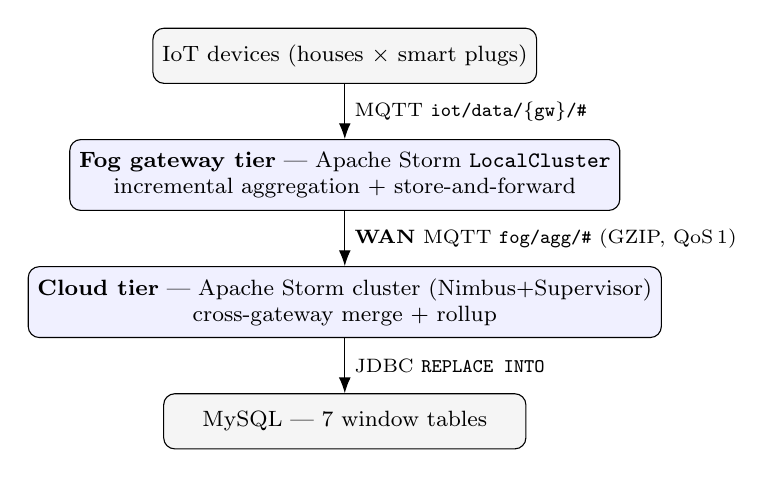
\begin{tikzpicture}[
  font=\footnotesize, >={Latex[length=2mm]},
  tier/.style={draw,rounded corners,minimum height=9mm,align=center,fill=blue!6,minimum width=66mm},
  dev/.style={draw,rounded corners,minimum height=7mm,align=center,fill=gray!8,minimum width=46mm}
]
\node[dev] (d1) {IoT devices (houses $\times$ smart plugs)};
\node[tier,below=7mm of d1] (gw) {\textbf{Fog gateway tier} --- Apache Storm \code{LocalCluster}\\incremental aggregation + store-and-forward};
\node[tier,below=7mm of gw] (cloud) {\textbf{Cloud tier} --- Apache Storm cluster (Nimbus+Supervisor)\\cross-gateway merge + rollup};
\node[dev,below=7mm of cloud] (db) {MySQL --- 7 window tables};
\draw[->] (d1) -- node[right,font=\scriptsize]{MQTT \code{iot/data/\{gw\}/\#}} (gw);
\draw[->] (gw) -- node[right,font=\scriptsize]{\textbf{WAN} MQTT \code{fog/agg/\#} (GZIP, QoS\,1)} (cloud);
\draw[->] (cloud) -- node[right,font=\scriptsize]{JDBC \code{REPLACE INTO}} (db);
\end{tikzpicture}
\caption{Migrated three-tier architecture. The gateway and cloud are independent
Storm deployments; only compressed aggregate batches cross the WAN.}
\label{fig:arch}
\end{figure}

\subsection{Fog Gateway Tier and Operator Redesign}\label{sec:arch-gw}
The gateway runs a Storm \code{LocalCluster} (single JVM, sized for a
Raspberry~Pi~3: \code{-Xmx384m}, serial GC). Its topology
(Fig.~\ref{fig:gwtopo}) has two spouts and one bolt:

\begin{itemize}
\item \textbf{\code{Spout\_rawData}} subscribes to \code{iot/data/\{gatewayId\}/\#}
  and emits each raw reading
  $(\textit{houseId},\textit{householdId},\textit{plugId},\textit{ts},
  \textit{value})$ on stream \code{data}, field-grouped by device key.
\item \textbf{\code{Spout\_trigger}} emits a pulse on stream \code{trigger} every
  $\Delta=\SI{60}{\second}$ (\code{FLUSH\_INTERVAL\_SEC}).
\item \textbf{\code{Bolt\_ingest}} (parallelism $1$) is the migrated operator. It
  replaces the original \code{split}$\to$\code{avg}$\to$\code{sum} chain.
\end{itemize}

The redesign is the heart of the migration. Rather than emit a tuple per window
into downstream bolts, \code{Bolt\_ingest} performs \emph{logical fan-out}: on
each \code{data} tuple it updates, for each of the $W=5$ windows
$\{1,5,10,15,30\}$ minutes, an in-memory accumulator
$\textsf{acc}[w][k]=(\textit{count},\textit{sum})$ keyed by
$k=\textit{house}{:}\textit{household}{:}\textit{plug}{:}\textit{date}{:}\textit{slice}$,
\emph{emitting no tuple}. Per-tuple work is therefore $O(W)$ in-memory updates
and $0$ network emissions, versus the original chain's per-window tuple
emissions. On a \code{trigger} tuple it calls \code{flush()}
(Algorithm~\ref{alg:flush}), which serializes each window's accumulators into one
\code{AggregatedBatch}, GZIP-compresses it, and publishes it to the cloud---or,
if the cloud is unreachable, appends it to a local disk queue.

Because count and sum are additive, the average the cloud later reconstructs,
$\overline{x}=\sum_i \textit{sum}_i / \sum_i \textit{count}_i$, equals the
monolithic average exactly (Section~\ref{sec:metrics}). The migration thus
preserves the analytics semantics of the original \code{avg}/\code{sum} bolts
while moving \emph{all} of that work to the edge and shipping only the compact
accumulator state.

\begin{figure}[t]
\centering
\resizebox{\columnwidth}{!}{%
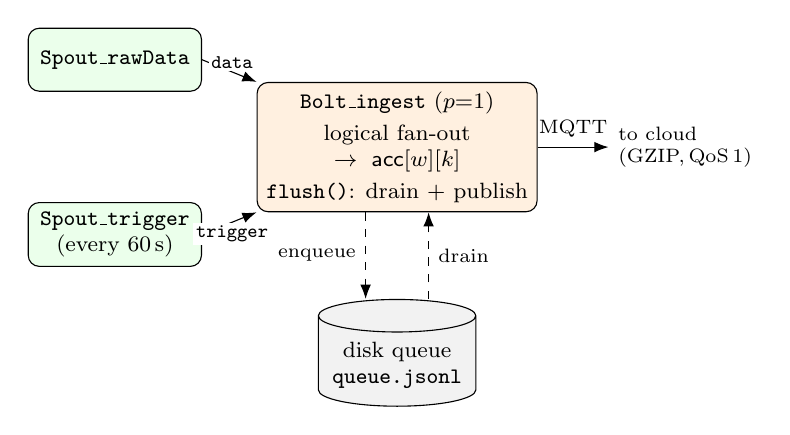
\begin{tikzpicture}[
  font=\footnotesize, >={Latex[length=1.8mm]},
  s/.style={draw,rounded corners,fill=green!8,align=center,minimum height=8mm,minimum width=22mm},
  b/.style={draw,rounded corners,fill=orange!12,align=center,minimum height=15mm,minimum width=32mm},
  q/.style={draw,cylinder,shape border rotate=90,aspect=0.22,fill=gray!10,align=center,
            minimum height=9mm,minimum width=20mm}
]
\node[s] (raw) {\code{Spout\_rawData}};
\node[s,below=14mm of raw] (trig) {\code{Spout\_trigger}\\(every \SI{60}{\second})};
\coordinate (mid) at ($(raw)!0.5!(trig)$);
\node[b,right=18mm of mid] (ingest)
  {\code{Bolt\_ingest} ($p{=}1$)\\[2pt]logical fan-out\\$\to\ \textsf{acc}[w][k]$\\[2pt]\code{flush()}: drain + publish};
\node[q,below=11mm of ingest] (q) {disk queue\\\code{queue.jsonl}};
\draw[->] (raw.east) -- node[pos=0.55,above,font=\scriptsize,fill=white,inner sep=1pt]{\code{data}} (ingest.north west);
\draw[->] (trig.east) -- node[pos=0.55,below,font=\scriptsize,fill=white,inner sep=1pt]{\code{trigger}} (ingest.south west);
\draw[->,dashed] ([xshift=-4mm]ingest.south) -- node[left,font=\scriptsize]{enqueue} ([xshift=-4mm]q.north);
\draw[->,dashed] ([xshift=4mm]q.north) -- node[right,font=\scriptsize]{drain} ([xshift=4mm]ingest.south);
\draw[->] (ingest.east) -- ++(9mm,0)
  node[midway,above,font=\scriptsize]{MQTT}
  node[right,align=left,font=\scriptsize]{to cloud\\(GZIP,\,QoS\,1)};
\end{tikzpicture}}
\caption{Fog gateway topology. \code{Bolt\_ingest} replaces the original
\code{split}$\to$\code{avg}$\to$\code{sum} chain: it aggregates in memory and, on
each trigger, drains the store-and-forward queue and publishes one compressed
batch per window.}
\label{fig:gwtopo}
\end{figure}

\begin{algorithm}[t]
\caption{\code{Bolt\_ingest.flush()} (per trigger)}
\label{alg:flush}
\begin{algorithmic}[1]
\STATE \code{drainQueue()} \hfill$\triangleright$ replay buffered batches first, QoS\,1
\FORALL{$w \in \{1,5,10,15,30\}$}
  \IF{$\textsf{acc}[w]$ non-empty}
    \STATE $B \gets \textsc{AggregatedBatch}(\textit{gwId},\textit{now},w,\textsf{acc}[w])$
    \STATE $p \gets \textsc{gzip}(\textsc{json}(B))$
    \IF{cloud MQTT connected}
      \STATE \code{publish}($p$, QoS\,1)
    \ELSE
      \STATE \code{appendToQueue}($\textsc{json}(B)$) \hfill$\triangleright$ disk persist
    \ENDIF
  \ENDIF
\ENDFOR
\STATE update capacity, EMA flush latency; clean stale slices
\end{algorithmic}
\end{algorithm}

\subsection{Cloud Tier}\label{sec:arch-cloud}
The cloud topology (Fig.~\ref{fig:cloudtopo}) mirrors the gateway shape but runs
as a full Storm cluster:

\begin{itemize}
\item \textbf{\code{Spout\_aggregated}} subscribes to \code{fog/agg/\#},
  GZIP-decompresses and deserializes each batch into an internal
  \code{LinkedBlockingQueue(10000)}, and emits it on stream \code{agg-data} with
  a message id $\textit{gwId}{:}\textit{ts}{:}w$ (so it is tracked by acking).
  Its \code{ack()}/\code{fail()} are no-ops: reliability is provided by MQTT QoS-1
  plus the gateway disk queue, not by Storm replay.
\item \textbf{\code{Spout\_trigger}} emits every \SI{60}{\second} on stream
  \code{trigger}, \emph{without} a message id (fire-and-forget): it is neither
  timed out nor throttled by \code{maxSpoutPending}.
\item \textbf{\code{Bolt\_cloudMerge}} (parallelism $1$, tagged \code{cloud})
  performs, on \code{agg-data}, a \code{REPLACE} of $\textsf{acc}[w][k]$ with the
  batch's cumulative values; on \code{trigger} it rolls up
  device~$\to$~household~$\to$~house, derives the 60- and 120-minute windows from
  the 30-minute data, and upserts all seven window tables via JDBC
  \code{REPLACE INTO}.
\end{itemize}

Running the merge as a separate single-instance bolt is what lets the cloud
\emph{unify} batches from all gateways (which are disjoint by \code{houseId},
hence conflict-free) without distributed coordination, and what lets the edge
keep operating independently when this tier is unreachable.

\begin{figure}[t]
\centering
\resizebox{\columnwidth}{!}{%
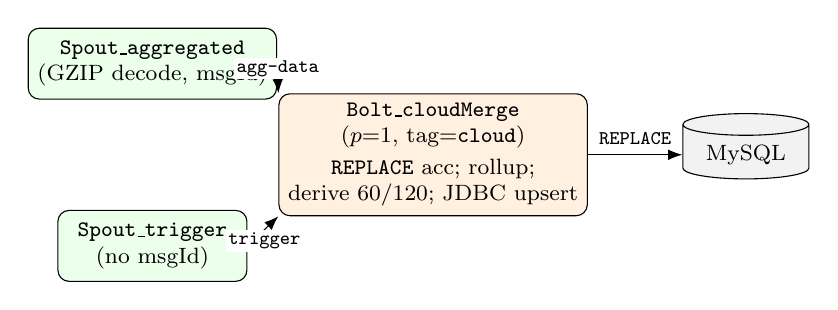
\begin{tikzpicture}[
  font=\footnotesize, >={Latex[length=1.8mm]},
  s/.style={draw,rounded corners,fill=green!8,align=center,minimum height=9mm,minimum width=24mm},
  b/.style={draw,rounded corners,fill=orange!12,align=center,minimum height=15mm,minimum width=34mm},
  db/.style={draw,cylinder,shape border rotate=90,aspect=0.22,fill=gray!10,align=center,
             minimum height=8mm,minimum width=16mm}
]
\node[s] (agg) {\code{Spout\_aggregated}\\(GZIP decode, msgId)};
\node[s,below=14mm of agg] (trig) {\code{Spout\_trigger}\\(no msgId)};
\coordinate (mid) at ($(agg)!0.5!(trig)$);
\node[b,right=16mm of mid] (merge)
  {\code{Bolt\_cloudMerge}\\($p{=}1$, tag=\code{cloud})\\[2pt]\code{REPLACE} acc; rollup;\\derive 60/120; JDBC upsert};
\node[db,right=12mm of merge] (db) {MySQL};
\draw[->] (agg.east) -- node[pos=0.55,above,font=\scriptsize,fill=white,inner sep=1pt]{\code{agg-data}} (merge.north west);
\draw[->] (trig.east) -- node[pos=0.55,below,font=\scriptsize,fill=white,inner sep=1pt]{\code{trigger}} (merge.south west);
\draw[->] (merge.east) -- node[above,font=\scriptsize]{\code{REPLACE}} (db.west);
\end{tikzpicture}}
\caption{Cloud topology. A single merge bolt, pinned to a supervisor tagged
\code{cloud}, unifies all gateways' batches; the untagged trigger drives the
periodic database write.}
\label{fig:cloudtopo}
\end{figure}

\subsection{Tier-Aware Scheduling}\label{sec:arch-sched}
Placement of operators onto tiers is delegated to the custom
\code{TagAwareScheduler} inherited from~\cite{pham2021}, an \code{IScheduler}
implementation invoked by Nimbus. It proceeds in three steps. (1) It groups
supervisors by the \code{tags} entry in their scheduler metadata
(\code{supervisor.scheduler.meta.tags} in \code{storm.yaml}); supervisors with no
tag fall into an \emph{untagged} group. (2) It groups topology components by the
\code{tags} field in each operator's JSON configuration, and---because Storm
internal components such as \code{\_\_acker} are not reachable through the
topology object---it folds those internals into the untagged group so they are
still placed. (3) For each tag, it collects the executors that need scheduling
and assigns them \emph{round-robin} across the available worker slots of the
supervisors carrying that tag; if any tag has executors but no available slot,
the entire scheduling fails atomically (avoiding a partial assignment).

In the migrated cloud topology, \code{Bolt\_cloudMerge} carries \code{tags=cloud}
and is therefore pinned to the supervisor whose \code{storm.yaml} declares
\code{supervisor.scheduler.meta.tags: cloud}; the spouts and the acker remain
untagged. This is the same tagging discipline the original used to scatter
\code{sum}/\code{forecast} to the cloud, but here it places a \emph{single,
self-contained} merge operator, so no per-tuple stream crosses the tier boundary
inside Storm---the only inter-tier traffic is the MQTT batch link.

\subsection{Store-and-Forward and Idempotent Replay}\label{sec:arch-saf}
Figure~\ref{fig:saf} shows the three store-and-forward phases. In steady state
each flush publishes directly. During a cloud outage, publishes fail and batches
are appended to \code{/var/fog-queue/\{gatewayId\}/queue.jsonl}; the gateway's own
ingestion is unaffected because \code{Bolt\_ingest} never blocks on the cloud. On
recovery, \code{drainQueue()} republishes buffered lines sequentially under
QoS-1, waiting for each broker acknowledgment before proceeding. Each batch
carries \emph{cumulative} totals for its slice, and the cloud applies
\code{REPLACE} (not add), so replaying a stale batch overwrites a key with an
equal-or-newer value:
\begin{equation}
\textsf{acc}[w][k] \;\leftarrow\; (\textit{count}_B,\ \textit{sum}_B),
\label{eq:replace}
\end{equation}
making replay \emph{idempotent}---no double counting after an arbitrarily long
outage. The MQTT client uses \code{MemoryPersistence} (avoiding a null-pointer
fault on Storm topology restart) and automatic reconnect.

\begin{figure}[t]
\centering
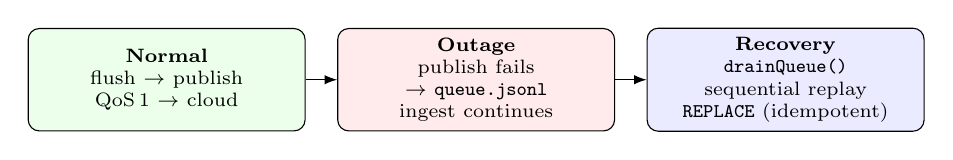
\begin{tikzpicture}[font=\scriptsize,node distance=4mm,>={Latex[length=1.6mm]},
  ph/.style={draw,rounded corners,minimum width=.29\linewidth,minimum height=13mm,align=center}]
\node[ph,fill=green!8] (n) {\textbf{Normal}\\flush $\to$ publish\\QoS\,1 $\to$ cloud};
\node[ph,fill=red!8,right=of n] (o) {\textbf{Outage}\\publish fails\\$\to$ \code{queue.jsonl}\\ingest continues};
\node[ph,fill=blue!8,right=of o] (r) {\textbf{Recovery}\\\code{drainQueue()}\\sequential replay\\\code{REPLACE} (idempotent)};
\draw[->] (n)--(o); \draw[->] (o)--(r);
\end{tikzpicture}
\caption{Store-and-forward phases. Gateway ingestion is decoupled from cloud
availability; recovery replays the disk queue idempotently.}
\label{fig:saf}
\end{figure}

\subsection{What the Migration Changes}\label{sec:arch-summary}
Table~\ref{tab:beforeafter} summarizes the before/after. The migration converts a
single tagged topology whose inter-tier traffic and fault behavior are coupled to
the device population into two independent topologies whose only link is a
constant-rate, compressed batch stream---preserving the analytics exactly while
decoupling WAN cost and cloud availability from scale.

\begin{table}[t]
\centering
\caption{Original cloud-centric design vs.\ migrated fog+cloud.}
\label{tab:beforeafter}
\footnotesize
\setlength{\tabcolsep}{3.5pt}
\begin{tabular}{p{2.5cm}p{2.5cm}p{2.5cm}}
\toprule
 & Original~\cite{pham2021} & Migrated (this work) \\
\midrule
Storm deployment & one tagged topology spanning tiers & two independent topologies \\
Edge operators & \code{split},\code{avg} (tagged gateway) & \code{Bolt\_ingest} (collapsed chain) \\
Cloud operators & \code{sum},\code{forecast} (tagged cloud) & \code{Bolt\_cloudMerge} \\
Inter-tier link & per-window tuple streams over WAN & one MQTT batch stream (GZIP) \\
WAN vs.\ devices & scales with device count & constant per gateway \\
Edge during outage & blocked (shared acker) & continues; disk queue \\
Replay safety & --- & idempotent \code{REPLACE} \\
\bottomrule
\end{tabular}
\end{table}

% ===========================================================================
\section{Validation Metric Definitions}\label{sec:metrics}
% ===========================================================================
We validate the migration with quantities measured directly by Storm's built-in
metrics or by an embedded Prometheus exporter on the gateway, scraped by
Prometheus and visualized in Grafana. This section gives each metric a closed
form so the validation is unambiguous.

\subsection{Offered Load}
With $N$ houses, each publishing at $s=10\msgps$, the offered load is
$\lambda = N \cdot s$. At $N=40$, $\lambda=400\msgps$ for both configurations.

\subsection{Aggregation Semantics and Algebraic Equivalence}
Each accumulator stores a (count, sum) pair. For window $w$ and device-slice key
$k$, the reconstructed average is
\begin{equation}
\overline{x}_{\text{fog}}(w,k)
 \;=\; \frac{\sum_{i} \textit{sum}_i}{\sum_{i} \textit{count}_i},
\label{eq:fogavg}
\end{equation}
where $i$ ranges over gateway batches contributing to $k$. Because count and sum
are additive, this equals the monolithic average
$\sum \textit{value}/N_{\text{samples}}$ exactly; the migrated edge operator
introduces no approximation relative to the original \code{avg}/\code{sum} bolts.
The derived long windows are obtained algebraically from the 30-minute slices,
\begin{equation}
\textit{slice}_{Wr} = \left\lfloor \textit{slice}_{30}/r \right\rfloor,\quad
r=W_r/30,
\label{eq:derive}
\end{equation}
with $(count,sum)$ summed over source slices mapping to the same derived slice
($r=2$ for 60-min, $r=4$ for 120-min), reproducing the monolithic slice index
since $\lfloor t/(60\!\cdot\!60000)\rfloor=\lfloor\lfloor t/(30\!\cdot\!60000)\rfloor/2\rfloor$.

\subsection{WAN Traffic and Reduction}
Let $b_{\text{raw}}$ be the wire size of one raw reading and $b_{\text{batch}}$
the compressed size of one aggregate batch ($b_{\text{batch}}\approx\SI{5}{\kilo\byte}$
in our deployment, vs.\ a few tens of bytes for $b_{\text{raw}}$). The original
cloud-centric path transmits $B_{\text{mono}} = \lambda \cdot 60 \cdot b_{\text{raw}}$
bytes/min, whereas the migrated fog path, flushing $W$ windows from $G$ gateways
once per minute, transmits $B_{\text{fog}} = G \cdot W \cdot b_{\text{batch}}$.
The WAN \emph{reduction} is
\begin{equation}
R \;=\; 1 - \frac{B_{\text{fog}}}{B_{\text{mono}}}.
\label{eq:wanred}
\end{equation}
We measure $B_{\text{fog}}$ in $\KBmin$ directly. The reported tuple
\emph{emitted}/\emph{transferred}/\emph{acked} reductions are each of the form
$1-(\text{aggregate count})/(\text{raw-ingress count})$, i.e.\ relative to the
system's own measured input (the volume a pass-through monolithic pipeline would
forward), not a separately deployed baseline.

\subsection{Bolt Execute Latency (EMA)}
The gateway exporter smooths per-tuple execute latency with an exponential moving
average (EMA),
\begin{equation}
\overline{\ell}_t = (1-\alpha)\,\overline{\ell}_{t-1} + \alpha\,\ell_t,
\label{eq:ema}
\end{equation}
with $\alpha=0.2$ for execute latency and $\alpha=0.3$ for flush latency.
Equation~\eqref{eq:ema} explains a non-obvious trend: at high $N$, hundreds of
fast sub-millisecond samples per second \emph{dilute} the rare flush spike, so the
reported gateway EMA \emph{decreases} as load rises.

\subsection{Bolt Capacity}
Storm defines bolt \emph{capacity} as the fraction of a measurement window the
bolt spent executing:
\begin{equation}
C \;=\; \frac{n_{\text{exec}}\cdot \overline{\ell}_{\text{exec}}}{T_{\text{win}}},
\label{eq:cap}
\end{equation}
with $n_{\text{exec}}$ tuples executed in window $T_{\text{win}}$ (we report the
rolling \SI{600}{\second} window). $C\to 1$ signals saturation. The gateway
exporter computes an analogous
$C_{\text{gw}}=\min(1, (m\cdot\overline{\ell})/T_{\text{win}})$, with $m$ tuples
processed in the flush window.

\subsection{Complete Latency and a Queueing Model}
Storm's \emph{complete latency} (CL) is the wall-clock time from a spout emitting
a tuple to the entire tuple tree being acked. For the cloud topology, CL is
dominated by the time an \code{agg-data} tuple waits for and is served by the
single merge bolt. Modeling that bolt as an M/M/1 server with mean service time
$E[S]$ and utilization $\rho=\lambda_{\text{eff}}E[S]$,
\begin{equation}
E[T] \;=\; \frac{E[S]}{1-\rho}.
\label{eq:mm1}
\end{equation}
Equation~\eqref{eq:mm1} is the lens for Section~\ref{sec:kb1}: packaging the same
data into fewer, heavier batches inflates $E[S]$, pushing $\rho$ toward $1$. We
use M/M/1 only as a first-order illustration; the actual arrivals are periodic
and bursty (a synchronized flush every $\Delta$) rather than Poisson, a
deterministic-arrival regime that only sharpens the effect.

\subsection{Store-and-Forward Queue, Recovery, and Loss}
During an outage of duration $t_{\text{out}}$, with flush interval $\Delta$, $W$
windows, and $G$ gateways, the maximum queue depth is
\begin{equation}
Q_{\max} \;=\; \left\lceil t_{\text{out}}/\Delta \right\rceil \cdot W \cdot G.
\label{eq:qmax}
\end{equation}
If recovery (queue returning to zero) takes $t_{\text{rec}}$, the drain rate and
per-batch drain time are
$r_{\text{drain}} = Q_{\max}/t_{\text{rec}}$ and
$\tau_{\text{batch}} = t_{\text{rec}}/Q_{\max}$.
Data loss is $L = 1 - (\#\text{drained})/(\#\text{enqueued})$.

% ===========================================================================
\section{Experimental Setup}\label{sec:setup}
% ===========================================================================
\textbf{Software.} Apache Storm~2.x; Eclipse Paho MQTT~1.2.5~\cite{eclipsepaho};
MySQL~8.0; Prometheus and Grafana; Docker Compose; Java~11; Maven. The gateway
runs as a Storm \code{LocalCluster}; the cloud runs a Storm cluster (one Nimbus,
one Supervisor) on an EC2 instance in \code{ap-southeast-1} (Singapore). The
gateway-to-cloud MQTT hop traverses the public WAN.

\textbf{Monolithic baseline.} As the ``before'' of the migration we measure the
original topology deployed \emph{cloud-only}: every raw reading is published
directly to a single cloud Storm cluster, where \code{Spout\_data} feeds
\code{Bolt\_split}, which fans out (all-grouping) into per-window
\code{Bolt\_avg}/\code{Bolt\_sum} chains over eight windows
$\{1,5,10,15,20,30,60,120\}$ minutes before acking back. Metrics are collected
with the same Storm exporter (\code{stormexporter:v1.2.2}, \SI{5}{\second} scrape)
into Prometheus/Grafana over a \SI{30}{\minute} window. This is the de-facto
starting configuration in which all aggregation runs centrally.

\textbf{Two fog configurations.} To then isolate the effect of \emph{batch
packaging}, the migrated fog deployments are physically identical except for how
the 40 houses are partitioned across gateways (Table~\ref{tab:env}).
\textsc{Env-A} distributes them over eight gateways (the migrated, fog-scaled
deployment); \textsc{Env-B} concentrates them on one gateway.

\begin{table}[t]
\centering
\caption{The two evaluated configurations.}
\label{tab:env}
\footnotesize
\begin{tabular}{lll}
\toprule
 & \textsc{Env-A} (distributed) & \textsc{Env-B} (centralized) \\
\midrule
Fog tier      & 8 containers (gw-01..08) & 1 container (gw-single) \\
Houses/gateway& 5                        & 40 \\
Cloud         & \multicolumn{2}{c}{EC2 Singapore, Storm (Nimbus+Supervisor)} \\
Monitoring    & \multicolumn{2}{c}{Prometheus ($8\times$ :9091) + Grafana} \\
Publisher     & \multicolumn{2}{c}{\code{send\_all.sh}, $N$ houses $\times 10\msgps$} \\
\bottomrule
\end{tabular}
\end{table}

\textbf{Scenarios.} \emph{KB1 (scalability)} ramps $N\in\{1,5,10,20,40\}$ houses,
\SI{300}{\second} per step, in both configurations (KB1-A, KB1-B). \emph{KB2
(fault tolerance)} fixes $N=40$ ($400\msgps$), warms up, takes the cloud MQTT
broker offline for \SI{300}{\second}, and measures recovery (KB2-A, KB2-B).

% ===========================================================================
\section{Validation: The Monolithic Baseline}\label{sec:mono}
% ===========================================================================
Before evaluating the migrated system we quantify the cloud-only baseline it
replaces. Table~\ref{tab:mono} reports its Storm metrics over the
\SI{30}{\minute} window. The central finding is a \emph{severe bottleneck}:
while most bolts run at capacity $<0.5$, the \code{avg-1} bolt---which recomputes
the shortest (1-minute) window and therefore fires most frequently---spikes to a
Storm capacity of \textbf{14.5} (Fig.~\ref{fig:mono-cap}). By
Eq.~\eqref{eq:cap}, $C=14.5$ means raw tuples arrive $14.5\times$ faster than the
single \code{avg-1} executor can drain them; the executor is in sustained overload
and the backlog grows. Consistent with this, the all-fan-out design emits
$\sim$\SI{6.5}{}~million and transfers $\sim$\SI{11}{}~million tuples in the window
(Fig.~\ref{fig:mono-et}; transferred $\approx 2\times$ emitted because
\code{Bolt\_split} uses all-grouping, so one emit becomes many inter-task
transfers), while only $\sim$\SI{11}{}~thousand \emph{root} tuples are acked. The
end-to-end complete latency reaches \SI{400}{}--\SI{550}{\milli\second} during
load, dominated by queuing at the bottleneck rather than CPU work (bolt
\emph{process} latency stays below \SI{1}{\milli\second}).

\begin{table}[t]
\centering
\caption{Monolithic cloud-only baseline (30-min window).}
\label{tab:mono}
\footnotesize
\begin{tabular}{lr}
\toprule
Metric (Storm exporter) & Value \\
\midrule
Acked (root tuples, all-time)      & $\sim$\num{11000} \\
Emitted (all-time)                 & $\sim$\SI{6.5}{}\,M \\
Transferred (all-time)             & $\sim$\SI{11}{}\,M \\
Bolt process latency               & $<\!\SI{1}{\milli\second}$ (spikes \SI{1.6}{\milli\second}) \\
Bolt execute latency               & baseline $\sim$\SI{25}{}, peak $\sim$\SI{60}{\milli\second} \\
\textbf{Bolt capacity (\code{avg-1})} & \textbf{14.5} (overload) \\
Topology complete latency          & \SI{400}{}--\SI{550}{\milli\second} (under load) \\
\bottomrule
\end{tabular}
\end{table}

\begin{figure}[t]
\centering
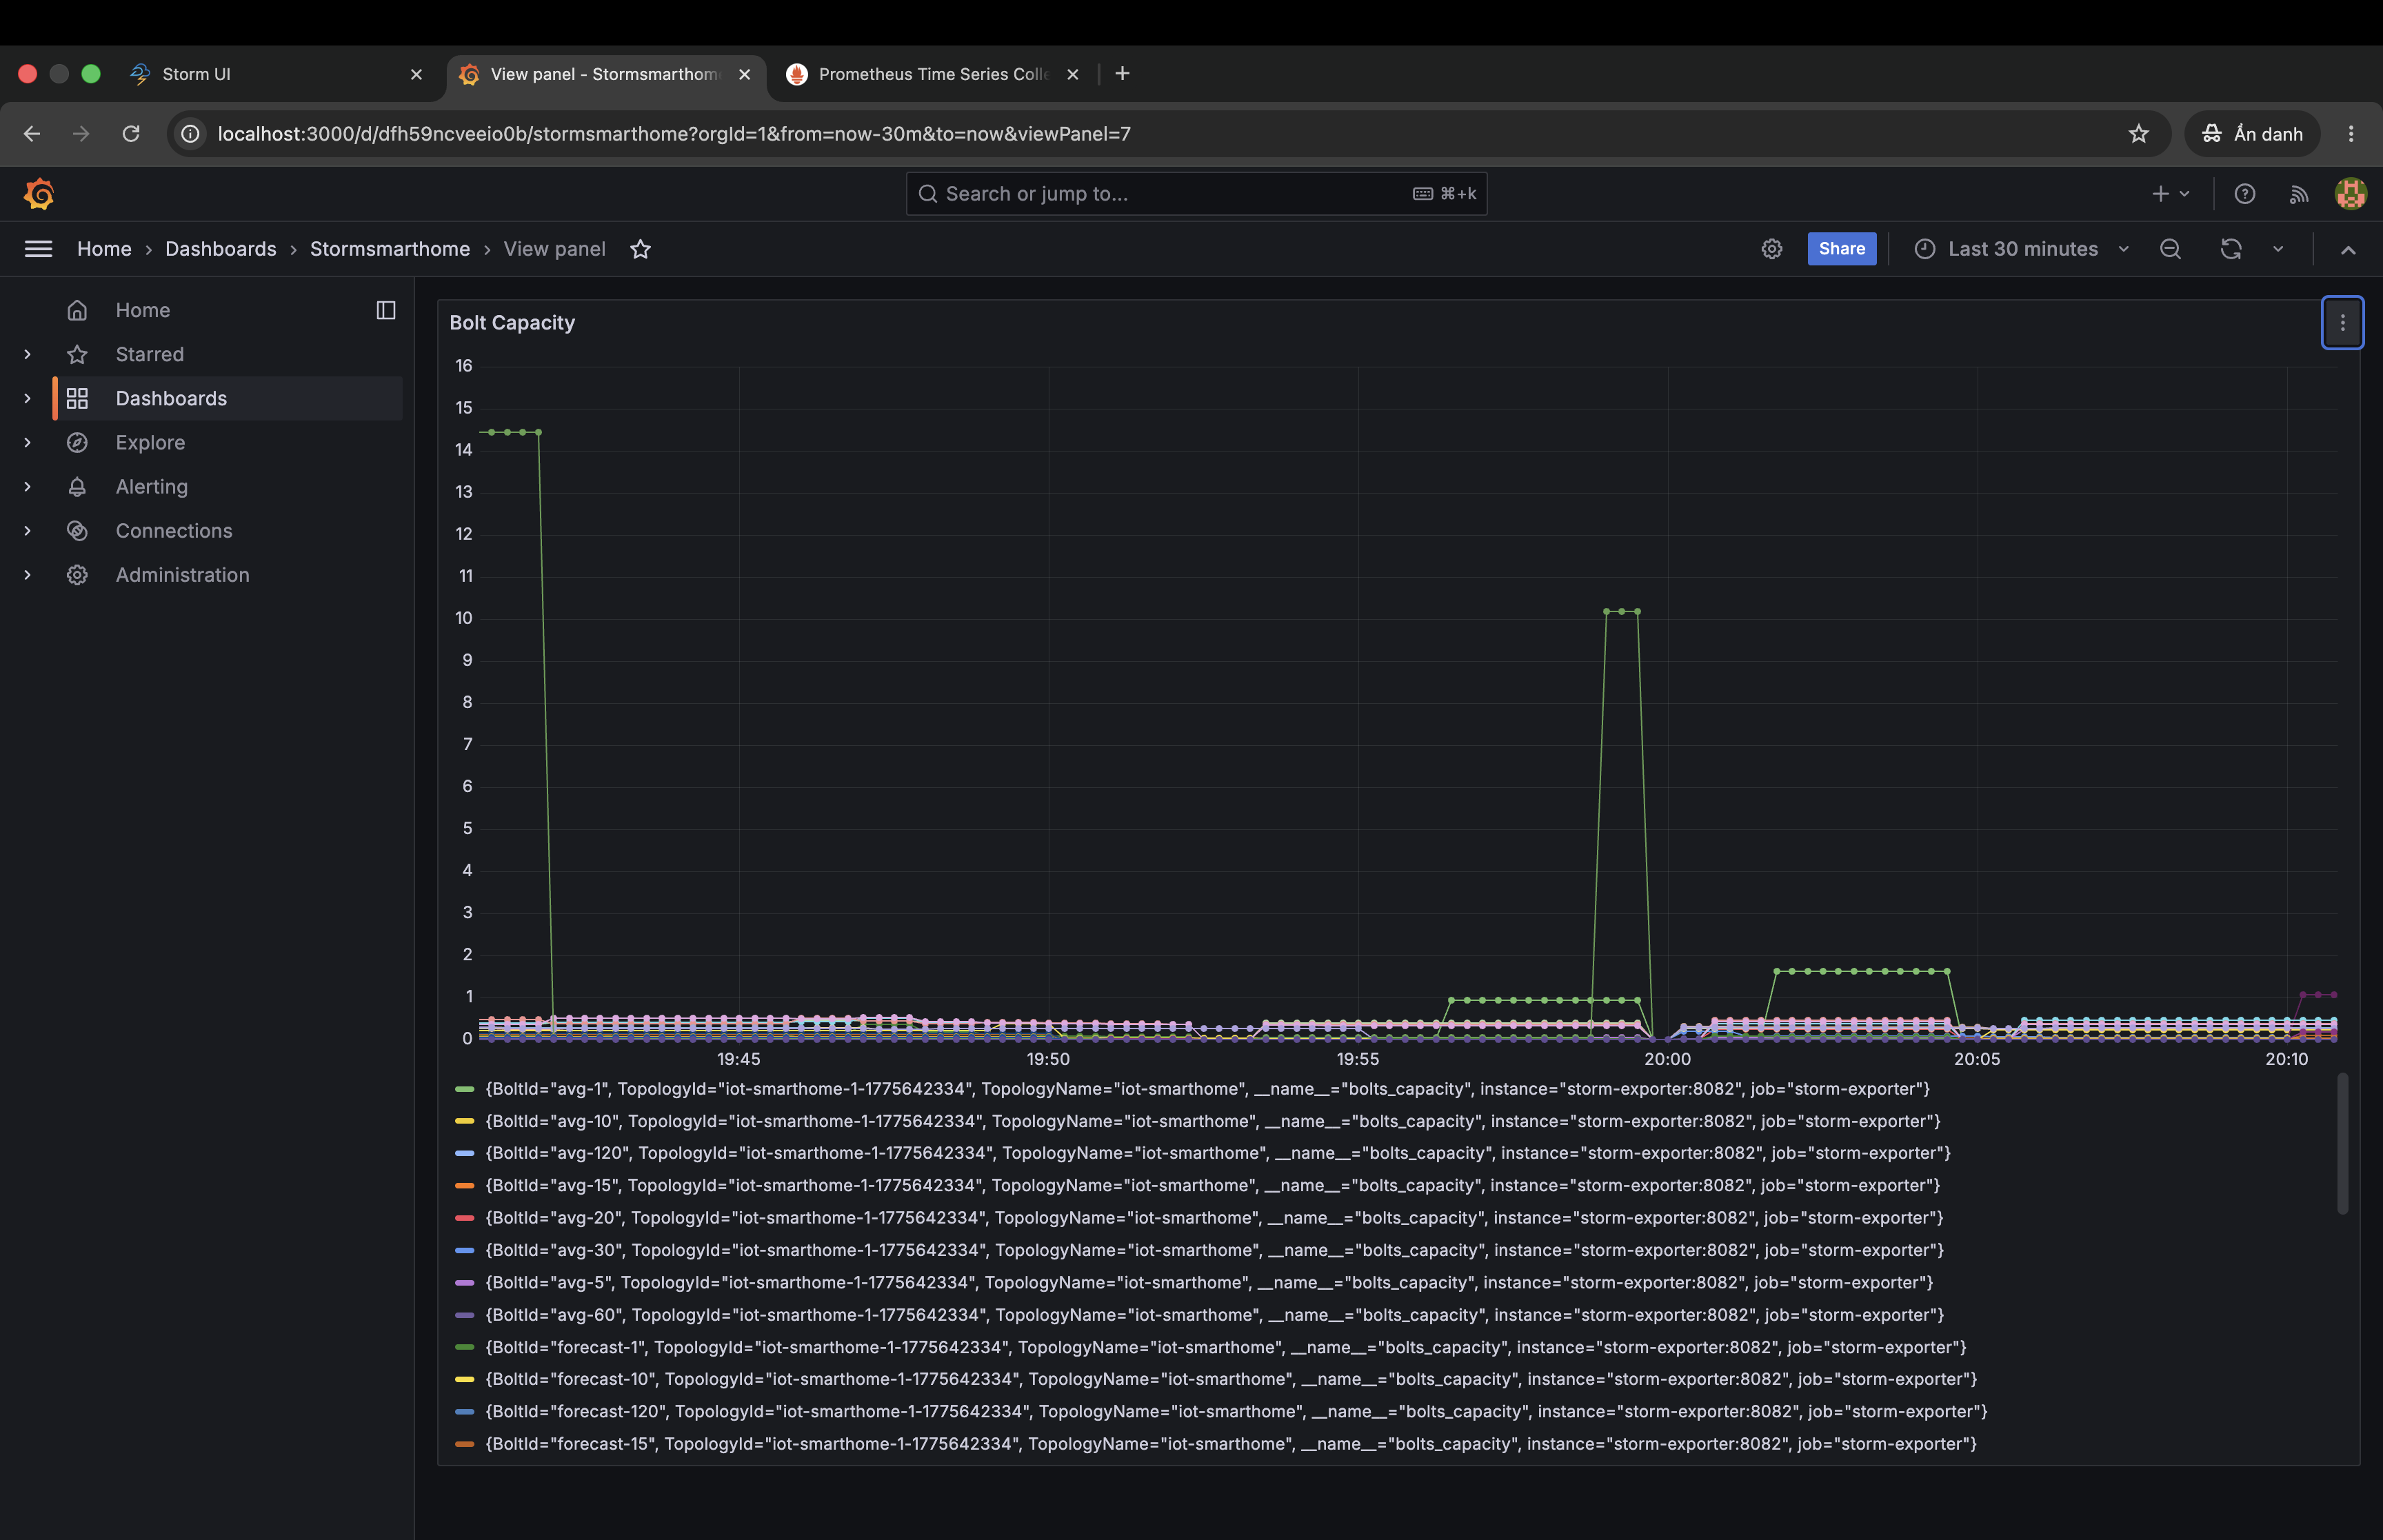
\includegraphics[width=\linewidth]{monolithic/mono_bolt_capacity.png}
\caption{Monolithic baseline bolt capacity. Most bolts sit below $0.5$, but
\code{avg-1} (green) spikes to \textbf{14.5}---the executor is $14.5\times$ over a
sustainable rate, the central bottleneck the migration removes.}
\label{fig:mono-cap}
\end{figure}

\begin{figure}[t]
\centering
\begin{subfigure}{0.49\linewidth}
  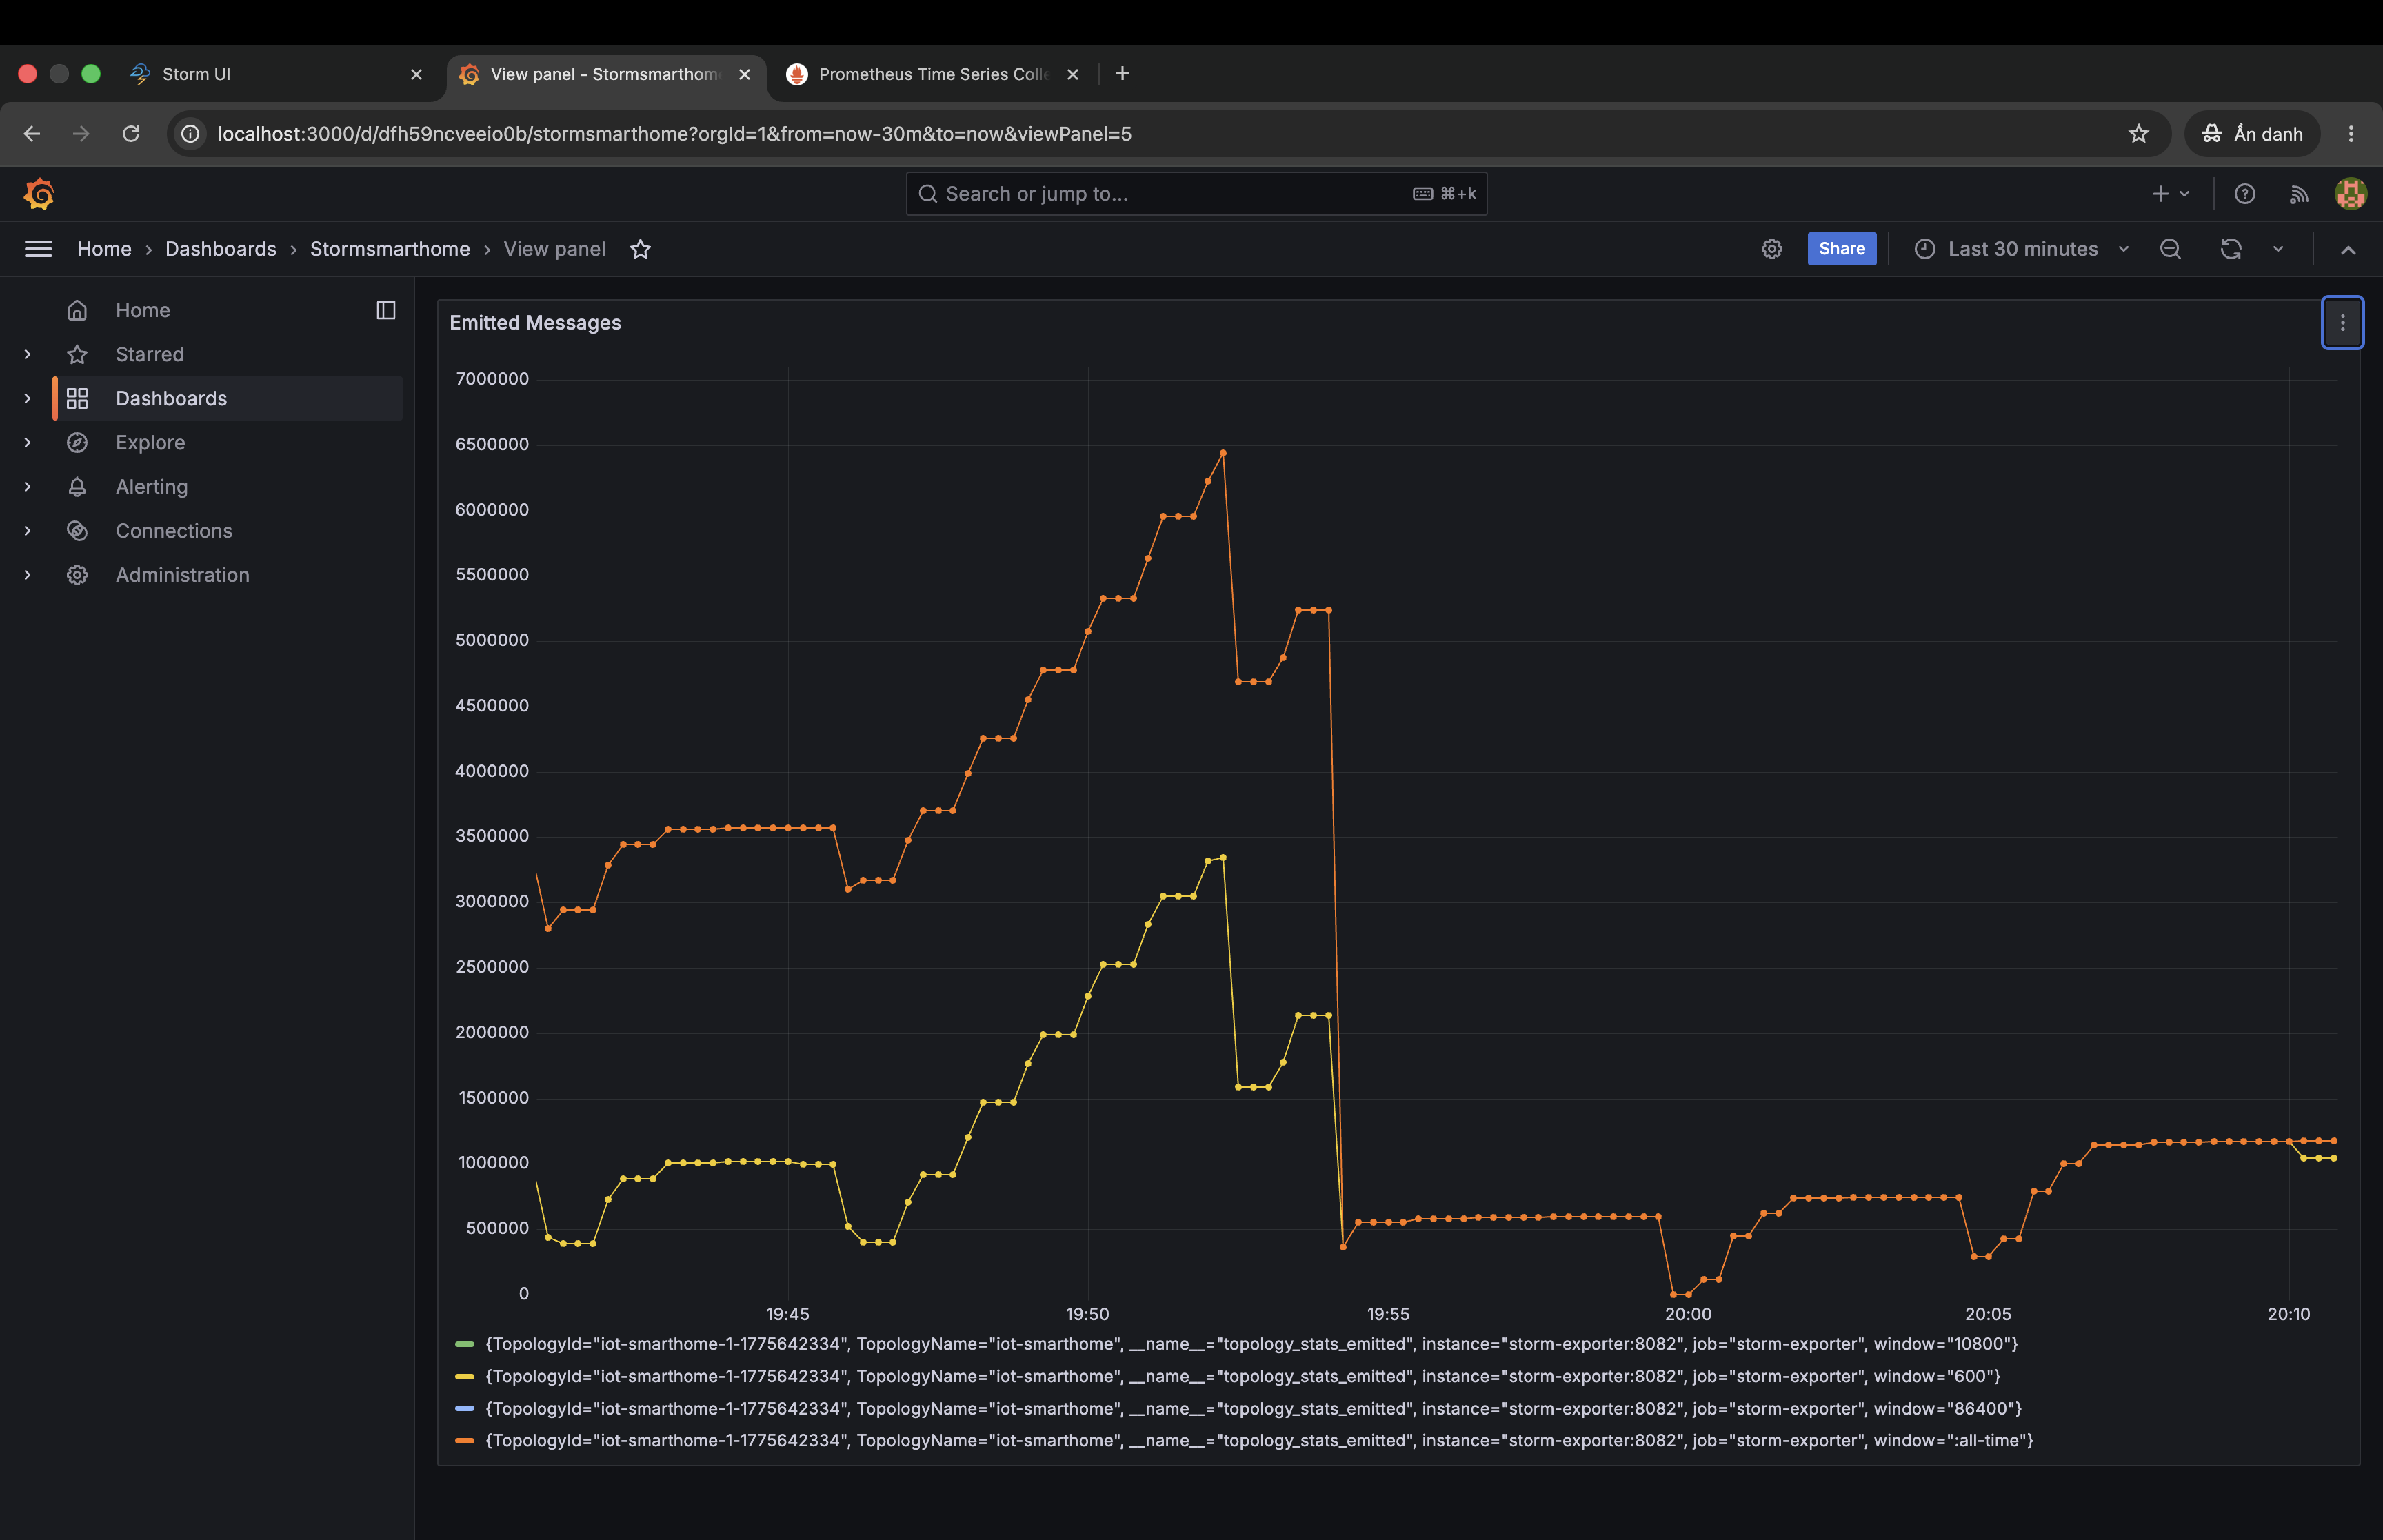
\includegraphics[width=\linewidth]{monolithic/mono_emitted.png}
  \caption{Emitted $\sim$\SI{6.5}{}\,M.}
\end{subfigure}\hfill
\begin{subfigure}{0.49\linewidth}
  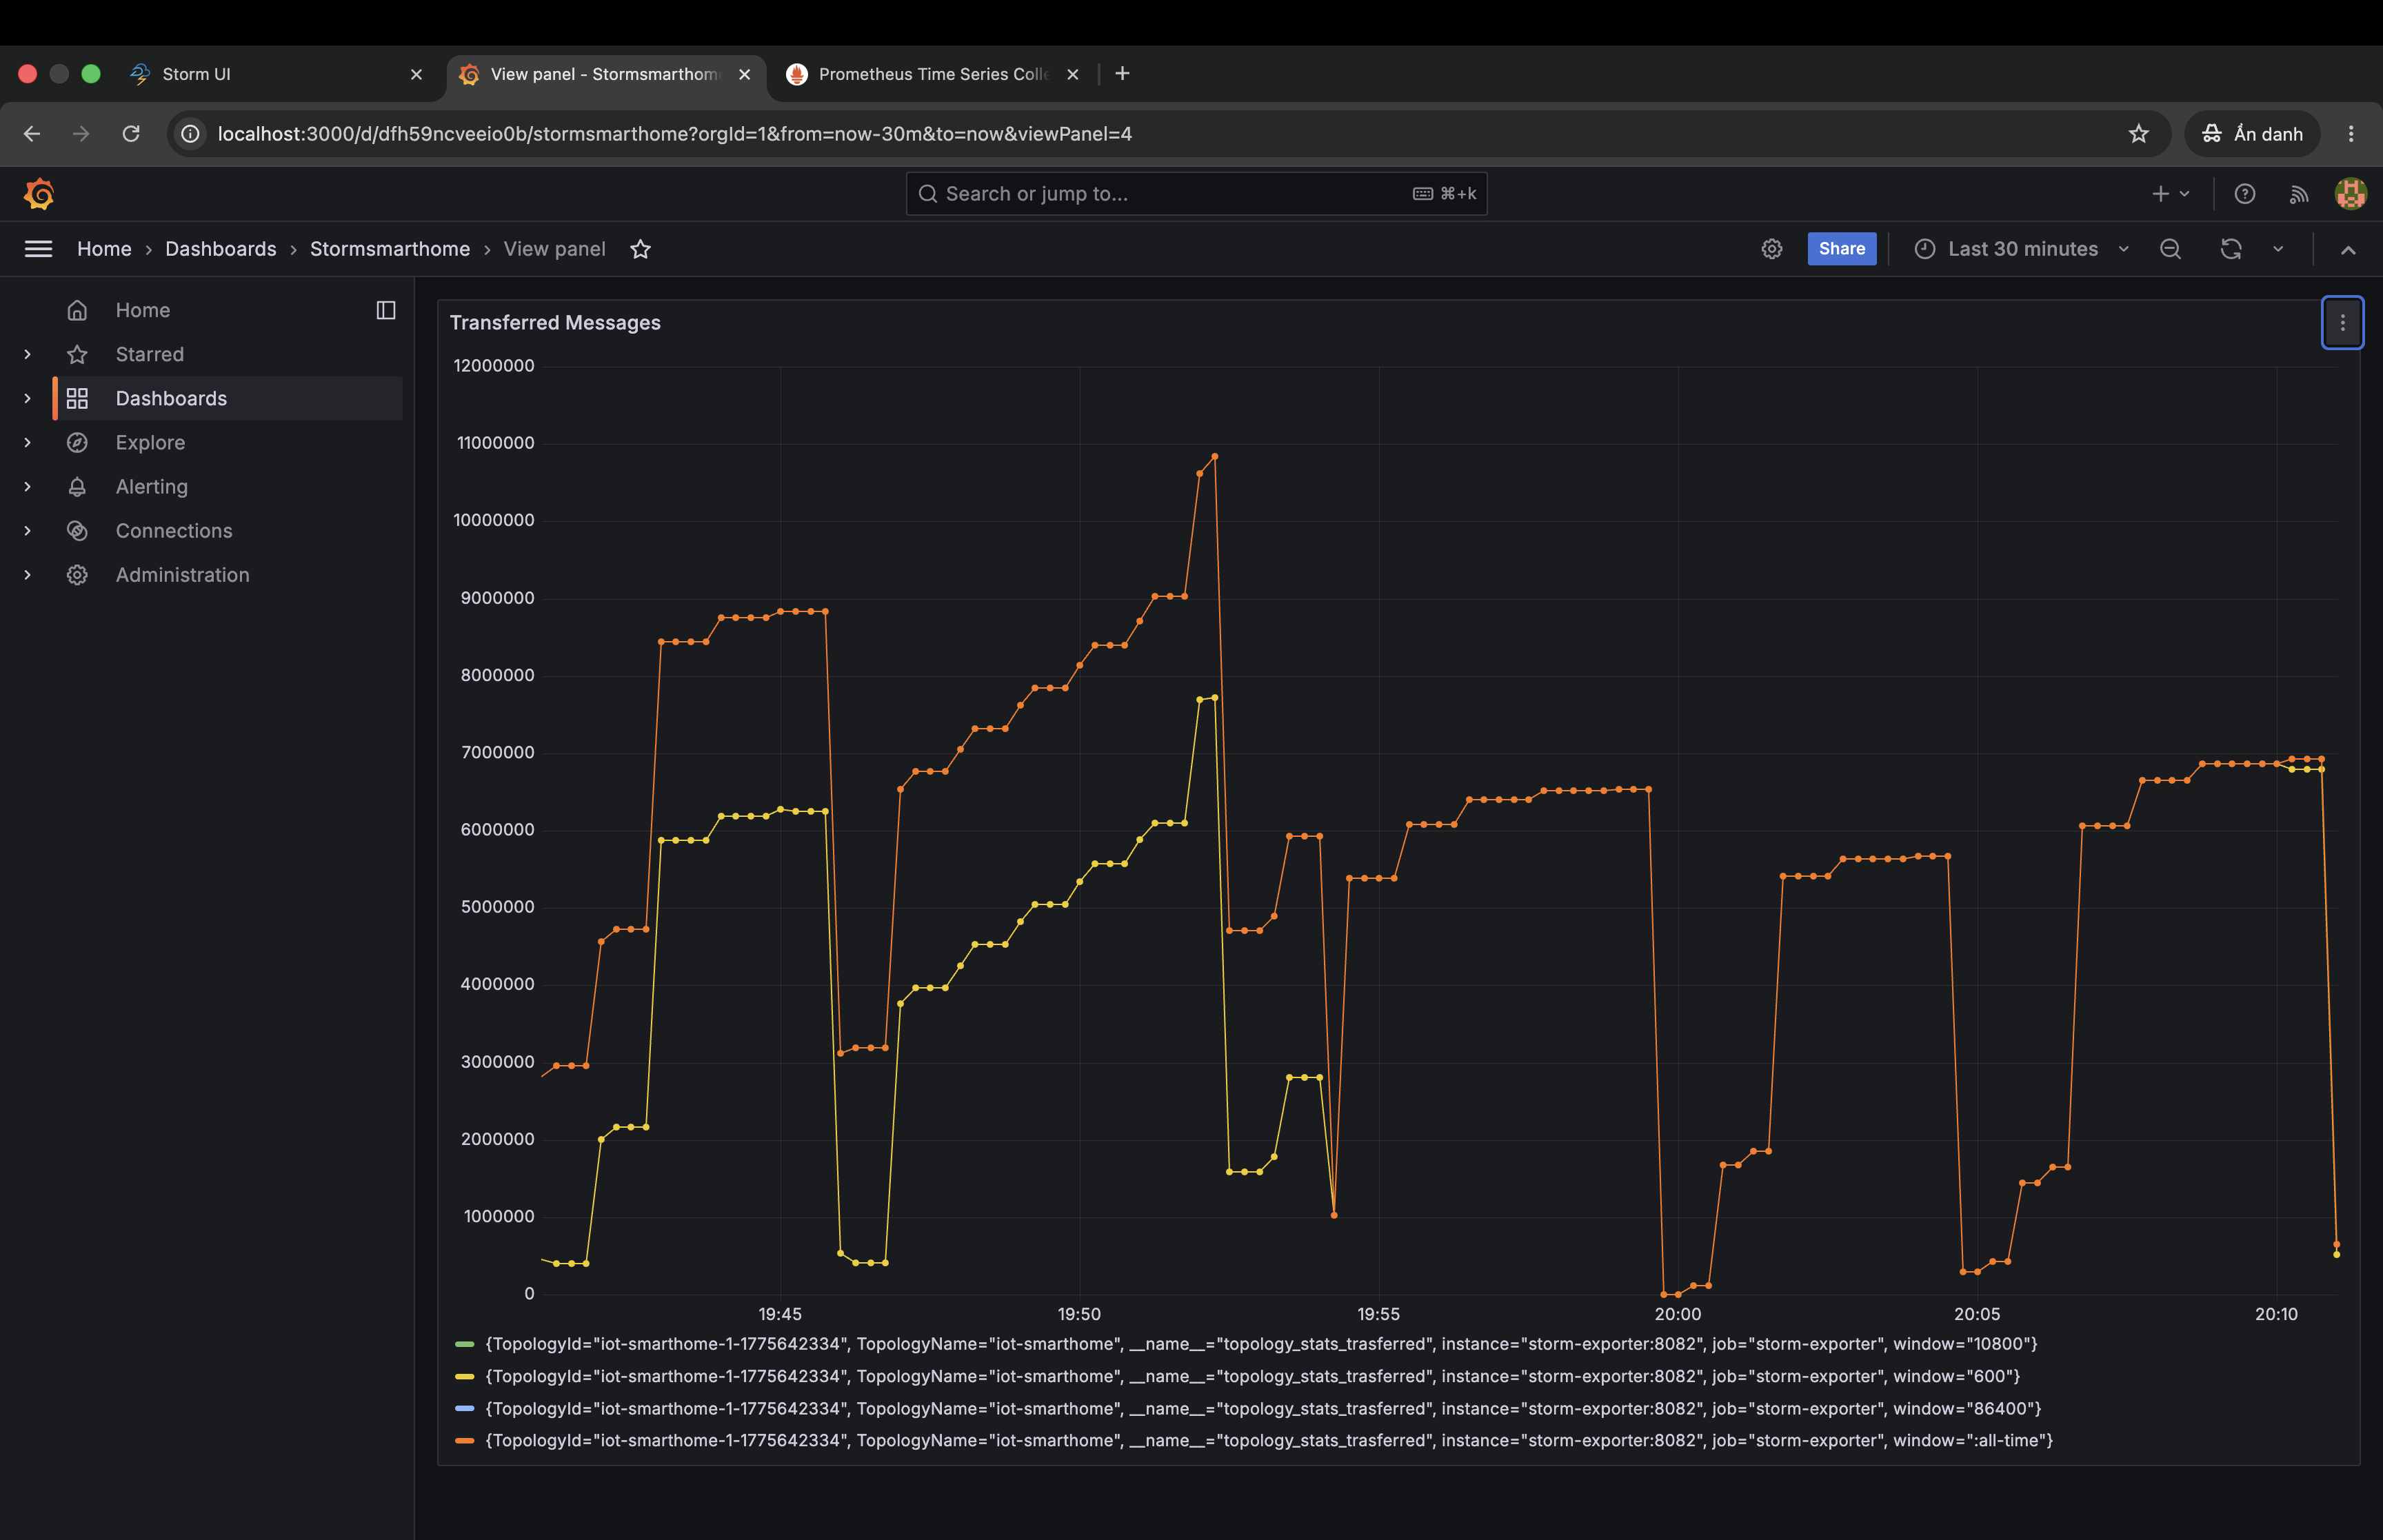
\includegraphics[width=\linewidth]{monolithic/mono_transferred.png}
  \caption{Transferred $\sim$\SI{11}{}\,M.}
\end{subfigure}
\caption{Monolithic baseline tuple volumes. Centralized fan-out over eight windows
inflates emitted and transferred tuples into the millions.}
\label{fig:mono-et}
\end{figure}

Table~\ref{tab:mono-vs-fog} contrasts the baseline with the migrated fog
deployment (\textsc{Env-A}, $N=40$). Moving the fan-out and windowing to the edge
collapses the cloud's intermediate tuple volumes by \SI{92}{}--\SI{93}{\percent}
and, decisively, removes the \code{avg-1} overload: the cloud merge bolt now runs
at capacity \num{0.245}. We note an honest caveat on complete latency: the
baseline's \SI{400}{}--\SI{550}{\milli\second} is measured over \emph{millions} of
raw tuples while the executor is at $14.5\times$ overload (an unsustainable regime
in which latency would diverge as load grows), whereas the fog cloud's
\SI{2439}{\milli\second} is measured over only $\sim$40 batch tuples per minute at
\SI{24.5}{\percent} capacity. The two are different tuple populations; the
meaningful gain is the elimination of the saturated bottleneck and the
order-of-magnitude reduction in intermediate work, not a per-tuple latency
comparison.

\begin{table}[t]
\centering
\caption{Monolithic cloud-only vs.\ migrated fog (\textsc{Env-A}, $N=40$).}
\label{tab:mono-vs-fog}
\footnotesize
\setlength{\tabcolsep}{3.5pt}
\begin{tabular}{lrrl}
\toprule
Metric & Monolithic & Fog (\textsc{Env-A}) & Change \\
\midrule
Emitted (cloud)        & $\sim$6.5\,M & --- & $-\SI{92.3}{\percent}$ \\
Transferred (cloud)    & $\sim$11\,M  & --- & $-\SI{92.5}{\percent}$ \\
Acked (cloud)          & $\sim$11\,k  & --- & $-\SI{85}{\percent}$ \\
Bolt capacity          & 14.5 (\code{avg-1}) & 0.245 (merge) & $59\times$ lower \\
Edge during outage     & n/a (cloud-only) & uninterrupted & --- \\
\bottomrule
\end{tabular}
\\[2pt]
\raggedright\scriptsize Reductions are the measured fog tuple
emitted/transferred/acked reductions (Section~\ref{sec:kb1}); the capacity ratio
compares the baseline's saturated \code{avg-1} executor with the fog cloud merge
bolt at $N=40$.
\end{table}

% ===========================================================================
\section{Validation: Fog Scalability}\label{sec:kb1}
% ===========================================================================
\subsection{Distributed Configuration (KB1-A)}
Table~\ref{tab:kb1a} reports KB1-A. Cloud complete latency \emph{saturates} at
$\approx\!\SI{2439}{\milli\second}$ from $N=20$ onward: it is bounded by the
once-per-minute MySQL write, not by $N$. Cloud bolt capacity rises only modestly
to \SI{24.5}{\percent} (rolling \SI{600}{\second}), with in-flush peaks near
\SI{48}{\percent}. The gateway bolt is never a bottleneck:
\SI{0.039}{\milli\second} per tuple across $N=5$--$40$, and its EMA \emph{falls}
with $N$ exactly as Eq.~\eqref{eq:ema} predicts. At $N=40$ the measured WAN
reductions are emitted $-\SI{92.3}{\percent}$, transferred $-\SI{92.5}{\percent}$,
acked $-\SI{85}{\percent}$ (Fig.~\ref{fig:kb1a-summary}).

\begin{table}[t]
\centering
\caption{KB1-A measurements (\textsc{Env-A}, 8 gateways).}
\label{tab:kb1a}
\setlength{\tabcolsep}{3.2pt}
\footnotesize
\begin{tabular}{rrrrrrr}
\toprule
$N$ & $\lambda$ & Cloud CL & Cloud & GW exec & GW flush & WAN \\
    & (msg/s)   & (ms)     & cap.  & (ms)    & (ms)     & (KB/min)\\
\midrule
1  & 10  & N/A$^{a}$ & N/A$^{b}$ & 0.027 & 56.4  & 14.1 \\
5  & 50  & 1738      & N/A$^{b}$ & 0.039 & 69.0  & 18.0 \\
10 & 100 & 2096      & 0.205     & 0.039 & 123.9 & 18.8 \\
20 & 200 & 2437      & 0.218     & 0.039 & 71.4  & 18.0 \\
40 & 400 & 2439      & 0.245     & 0.039 & 205.2 & 18.4 \\
\bottomrule
\end{tabular}
\\[2pt]
\raggedright\scriptsize $^{a}$Topology not yet stable at start.
$^{b}$Exporter field-transposition bug at low $N$. Gateway CPU stayed
$<\!\SI{27}{\percent}$ and RAM \SIrange{183}{203}{\mega\byte}; the
\SI{90.2}{\percent} CPU reading at $N{=}40$ is a single-host artifact of eight
containers flushing simultaneously, not representative load.
\end{table}

\begin{figure}[t]
\centering

\includegraphics[width=\linewidth]{kb1-A-multi8gw/summary_stat_panels.png}
\caption{KB1-A summary panels (\textsc{Env-A}, $N=40$): measured WAN reductions
of \SI{85}{\percent} acked, \SI{92.3}{\percent} emitted, \SI{92.5}{\percent}
transferred.}
\label{fig:kb1a-summary}
\end{figure}

\begin{figure}[t]
\centering
\begin{subfigure}{\linewidth}
  
\includegraphics[width=\linewidth]{kb1-A-multi8gw/cloud_bolt_execute_latency_ms.png}
  \caption{Execute latency saturates near \SI{5}{\second}.}
\end{subfigure}\\[2pt]
\begin{subfigure}{\linewidth}
  
\includegraphics[width=\linewidth]{kb1-A-multi8gw/cloud_bolt_capacity_600s.png}
  \caption{Capacity climbs slowly, saturating near \SI{24.5}{\percent}.}
\end{subfigure}
\caption{KB1-A cloud bolt behavior as $N$ ramps. Both quantities plateau,
confirming the database-write ceiling rather than an $N$-dependent bottleneck.}
\label{fig:kb1a-cloud}
\end{figure}

\subsection{Centralized Configuration (KB1-B)}
Table~\ref{tab:kb1b} reports KB1-B. Here cloud complete latency grows
\emph{near-linearly}, increasing \SI{63}{}--\SI{79}{\percent} on each doubling of
$N$ and reaching \SI{77006}{\milli\second} at $N=40$, because a single gateway
packs all $N$ houses into one batch per window, so the single-threaded merge bolt
blocks longer per tuple (Eq.~\eqref{eq:mm1} with growing $E[S]$). Cloud capacity
climbs to \SI{76.5}{\percent} (peak \SI{88.5}{\percent}) without saturating, and
WAN traffic grows $\approx\!26\times$ from $N=1$ to $N=40$ because the single
batch payload is proportional to $N$. The gateway itself stays idle
(\SI{10}{}--\SI{11}{\percent} CPU, no loss).

\begin{table}[t]
\centering
\caption{KB1-B measurements (\textsc{Env-B}, 1 gateway).}
\label{tab:kb1b}
\setlength{\tabcolsep}{3.2pt}
\footnotesize
\begin{tabular}{rrrrrrr}
\toprule
$N$ & $\lambda$ & Cloud CL & Cloud & GW exec & GW flush & WAN \\
    & (msg/s)   & (ms)     & cap.  & (ms)    & (ms)     & (KB/min)\\
\midrule
1  & 10  & 11006 & 0.223 & 0.023 & 328.7 & 8.2   \\
5  & 50  & 15470 & 0.299 & 0.034 & 333.8 & 25.6  \\
10 & 100 & 25232 & 0.488 & 0.026 & 358.2 & 51.8  \\
20 & 200 & 43090 & 0.710 & 0.023 & 373.0 & 107.0 \\
40 & 400 & 77006 & 0.765 & 0.012 & 412.4 & 213.7 \\
\bottomrule
\end{tabular}
\end{table}

\begin{figure}[t]
\centering
\begin{subfigure}{\linewidth}
  
\includegraphics[width=\linewidth]{kb1-B-single/cloud_bolt_execute_latency_ms.png}
  \caption{Execute latency grows from \SI{11}{} to \SI{77}{\second}.}
\end{subfigure}\\[2pt]
\begin{subfigure}{\linewidth}
  
\includegraphics[width=\linewidth]{kb1-B-single/cloud_bolt_capacity_600s.png}
  \caption{Capacity climbs to \SI{76.5}{\percent} without plateauing.}
\end{subfigure}
\caption{KB1-B cloud bolt behavior. Unlike KB1-A, both quantities scale with $N$:
the heavy single batch keeps the merge bolt busy.}
\label{fig:kb1b-cloud}
\end{figure}

\subsection{Head-to-Head at $N=40$}
Table~\ref{tab:headtohead} and Figs.~\ref{fig:cl-vs-n}--\ref{fig:wan-vs-n}
compare the two at identical load. Both ship the same information and achieve the
same $\approx\!\SI{92}{\percent}$ WAN-reduction \emph{shape}; the differences are
purely from packaging.

\begin{table}[t]
\centering
\caption{\textsc{Env-A} vs.\ \textsc{Env-B} at $N=40$ ($400\msgps$).}
\label{tab:headtohead}
\footnotesize
\begin{tabular}{lrrr}
\toprule
Metric & \textsc{Env-A} & \textsc{Env-B} & Ratio \\
\midrule
Cloud complete latency (ms)      & 2439  & 77006 & $31.6\times$ \\
Cloud capacity (600\,s avg)      & 0.245 & 0.765 & $3.1\times$ \\
Cloud max execute latency (s)    & 4.8   & 12.3  & $2.6\times$ \\
WAN (KB/min)                     & 18    & 213   & $11.6\times$ \\
Gateway CPU (per node)           & $\ll\!10\%^{*}$ & 10.6\% & $\approx$ \\
Data loss                        & 0\%   & 0\%   & --- \\
\bottomrule
\end{tabular}
\\[2pt]
\raggedright\scriptsize $^{*}$The \SI{90.2}{\percent} aggregate reading in
\textsc{Env-A} is a single-host artifact (eight containers flushing at once on one
machine), not per-node load.
\end{table}

\begin{figure}[t]
\centering
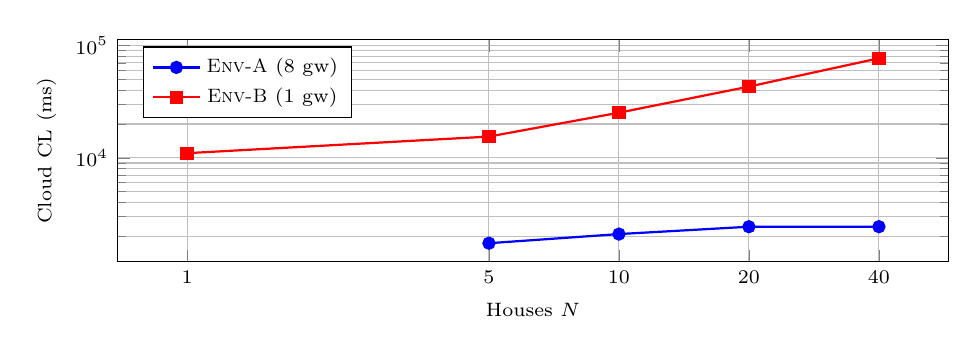
\begin{tikzpicture}
\begin{axis}[width=\linewidth,height=4.4cm,xlabel={Houses $N$},
  ylabel={Cloud CL (ms)},xmode=log,ymode=log,log basis x=2,
  xtick={1,5,10,20,40},xticklabels={1,5,10,20,40},
  legend pos=north west,legend style={font=\scriptsize},
  grid=both,tick label style={font=\scriptsize},label style={font=\scriptsize}]
\addplot[mark=*,thick,blue] coordinates {(5,1738)(10,2096)(20,2437)(40,2439)};
\addplot[mark=square*,thick,red] coordinates {(1,11006)(5,15470)(10,25232)(20,43090)(40,77006)};
\legend{\textsc{Env-A} (8 gw),\textsc{Env-B} (1 gw)}
\end{axis}
\end{tikzpicture}
\caption{Cloud complete latency vs.\ $N$ (log--log). \textsc{Env-A} is flat
(database-bound); \textsc{Env-B} grows near-linearly (batch-bound), $31.6\times$
higher at $N=40$.}
\label{fig:cl-vs-n}
\end{figure}

\begin{figure}[t]
\centering
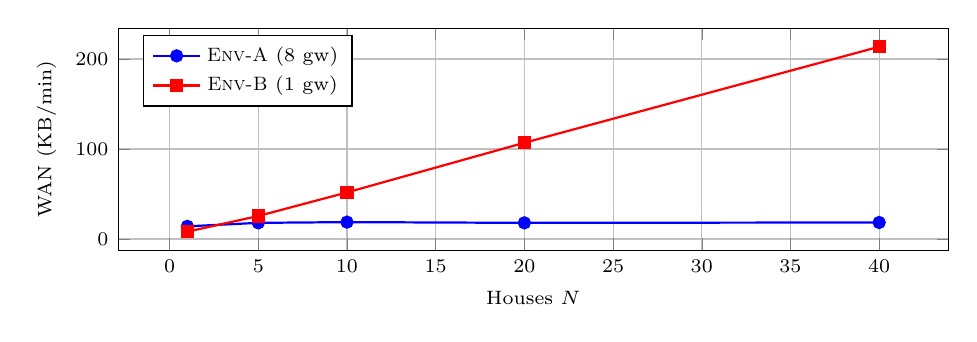
\begin{tikzpicture}
\begin{axis}[width=\linewidth,height=4.4cm,xlabel={Houses $N$},
  ylabel={WAN (KB/min)},legend pos=north west,
  legend style={font=\scriptsize},grid=both,
  tick label style={font=\scriptsize},label style={font=\scriptsize}]
\addplot[mark=*,thick,blue] coordinates {(1,14.1)(5,18.0)(10,18.8)(20,18.0)(40,18.4)};
\addplot[mark=square*,thick,red] coordinates {(1,8.2)(5,25.6)(10,51.8)(20,107.0)(40,213.7)};
\legend{\textsc{Env-A} (8 gw),\textsc{Env-B} (1 gw)}
\end{axis}
\end{tikzpicture}
\caption{WAN traffic vs.\ $N$. \textsc{Env-A} is flat at $\approx\!18\KBmin$;
\textsc{Env-B} grows linearly because one gateway's batch payload scales with $N$.}
\label{fig:wan-vs-n}
\end{figure}

\textbf{Mechanism.} With eight gateways, each flush produces eight \emph{small}
MQTT messages; the merge bolt processes light tuples and returns to idle quickly,
so the untracked trigger is served promptly and CL stays low. With one gateway,
each flush produces one \emph{heavy} message per window; the merge bolt blocks,
the trigger waits behind it, and CL escalates through queueing
(Eq.~\eqref{eq:mm1}). This is an \emph{architectural} property of batch size, not
an artifact of the scheduler. We caution that the $31.6\times$ \emph{magnitude} is
specific to this implementation---the merge bolt is single-threaded and opens
fresh JDBC connections per trigger (limit L1, Section~\ref{sec:limits}); a pooled
or partitioned merge would lower $E[S]$ and shrink the gap. The \emph{direction}
of the effect is structural and would persist.

% ===========================================================================
\section{Validation: Fault Tolerance}\label{sec:kb2}
% ===========================================================================
\subsection{Distributed Recovery (KB2-A)}
With the cloud broker offline for \SI{300}{\second}, KB2-A accumulated a maximum
queue depth of \textbf{200 batches}, matching Eq.~\eqref{eq:qmax} exactly:
$\lceil 300/60\rceil \cdot 5 \cdot 8 = 200$. After the cloud returned, the queue
drained to zero in $t_{\text{rec}}=\SI{71}{\second}$
($r_{\text{drain}}=200/71=2.8$ batch/s, $4.2\times$ faster than the
accumulation rate $0.67$ batch/s). Loss was $L=0$ (200 enqueued, 200 drained).
The gateway processed \num{102615} tuples during the outage without interruption
(Fig.~\ref{fig:kb2-queue} left; Fig.~\ref{fig:kb2-ingest}). The post-recovery
flood pushed cloud execute latency from $\approx\!\SI{4.8}{\second}$ to
\SI{25}{}--\SI{28}{\second} and capacity to \SI{80}{}--\SI{95}{\percent}, while
gateway latency stayed sub-millisecond. Because of \code{REPLACE} semantics
(Eq.~\eqref{eq:replace}), the post-recovery database write is the same size as in
steady state---no data amplification.

\subsection{Centralized Recovery (KB2-B)}
KB2-B accumulated only \textbf{25 batches}
($\lceil 300/60\rceil \cdot 5 \cdot 1$) yet recovered \emph{slower}, in
$t_{\text{rec}}=\SI{101}{\second}$. This is the \textbf{recovery paradox}: despite
an $8\times$ smaller queue, recovery is \SI{42}{\percent} longer. The per-batch
drain time makes the cause explicit: $\tau_{\text{batch}}=101/25=\SI{4.0}{\second}$
for \textsc{Env-B} vs.\ $71/200=\SI{0.35}{\second}$ for \textsc{Env-A}---an
$11.4\times$ heavier cost per batch. Both carry the same backlog
($200\times 5 = 25\times 40 = 1000$ house-records), but \code{drainQueue()}
publishes sequentially and waits for each QoS-1 acknowledgment, so the larger
40-house payload is acknowledged more slowly. The cloud overload is worse: execute
latency peaked at \textbf{\SI{2.03}{\minute}} (vs.\ \SI{26.8}{\second}) and
capacity hit \textbf{\SI{101}{\percent}} (vs.\ \SI{80.3}{\percent}), the latter
exceeding saturation because each tuple carries 40 houses and the untracked
trigger keeps injecting work while the bolt is busy. The gateway again never
stalled (\num{110846} tuples, $\approx\!260$ tuples/s).

\begin{table}[t]
\centering
\caption{KB2-A vs.\ KB2-B recovery.}
\label{tab:kb2}
\footnotesize
\begin{tabular}{lrr}
\toprule
Metric & KB2-A (8 gw) & KB2-B (1 gw) \\
\midrule
Max queue depth (batches)     & 200    & 25 \\
Recovery time (s)             & 71     & 101 \\
Per-batch drain time (s)      & 0.35   & 4.0 \\
Drain rate (batch/s)          & 2.8    & 0.25 \\
Cloud max execute latency     & 26.8\,s & 2.03\,min \\
Cloud max capacity            & 80.3\% & 101\% \\
Data loss                     & 0\%    & 0\% \\
Gateway interrupted           & no     & no \\
\bottomrule
\end{tabular}
\end{table}

\begin{figure}[t]
\centering
\begin{subfigure}{0.49\linewidth}
  
\includegraphics[width=\linewidth]{kb2-A-multi8gw/gateway_store_forward_queue_depth.png}
  \caption{KB2-A: $0\!\to\!200\!\to\!0$, \SI{71}{\second}.}
\end{subfigure}\hfill
\begin{subfigure}{0.49\linewidth}
  
\includegraphics[width=\linewidth]{kb2-B-single/gateway_store_forward_queue_depth.png}
  \caption{KB2-B: $0\!\to\!25\!\to\!0$, \SI{101}{\second}.}
\end{subfigure}
\caption{Store-and-forward queue depth during the \SI{300}{\second} outage and
recovery. The smaller \textsc{Env-B} queue drains more slowly per batch.}
\label{fig:kb2-queue}
\end{figure}

\begin{figure}[t]
\centering

\includegraphics[width=\linewidth]{kb2-A-multi8gw/gateway_tuple_ingestion_rate.png}
\caption{KB2-A gateway ingestion is uninterrupted throughout the cloud outage:
the fog tier is decoupled from cloud availability.}
\label{fig:kb2-ingest}
\end{figure}

\begin{figure}[t]
\centering
\begin{subfigure}{0.49\linewidth}
  
\includegraphics[width=\linewidth]{kb2-A-multi8gw/cloud_bolt_capacity_600s.png}
  \caption{KB2-A: \SI{80}{}--\SI{95}{\percent}.}
\end{subfigure}\hfill
\begin{subfigure}{0.49\linewidth}
  
\includegraphics[width=\linewidth]{kb2-B-single/cloud_bolt_capacity_600s.png}
  \caption{KB2-B: reaches \SI{101}{\percent}.}
\end{subfigure}
\caption{Cloud bolt capacity during the post-recovery flood. The centralized
configuration's heavier replayed batches drive the merge bolt past saturation.}
\label{fig:kb2-cap}
\end{figure}

% ===========================================================================
\section{Discussion}\label{sec:discussion}
% ===========================================================================
\subsection{What the Migration Buys}
The validation confirms the two properties the migration set out to fix.
\emph{(i) WAN decoupled from device count}: in \textsc{Env-A} the fog tier holds
WAN traffic flat at $\approx\!18\KBmin$ (a \SI{92}{}--\SI{93}{\percent} reduction;
Fig.~\ref{fig:wan-vs-n}) regardless of $N$, because only constant-rate compressed
batches cross the WAN---unlike the original coupled topology whose inter-tier
streams scale with devices. \emph{(ii) Edge autonomy}: across the full
\SI{300}{\second} outage the gateway never paused (Fig.~\ref{fig:kb2-ingest}) and
lost no data, because the migrated edge operator is self-contained and disk-backed
rather than sharing an acker with cloud operators. The migration also leaves the
analytics numerically identical (Eq.~\eqref{eq:fogavg}).

Crucially, the migration removes the baseline's central bottleneck: the
cloud-only \code{avg-1} executor ran at capacity $14.5$
(Fig.~\ref{fig:mono-cap}), i.e.\ $14.5\times$ over a sustainable rate, whereas
after moving all windowing and fan-out to the edge the cloud merge bolt runs at
$0.245$ ($N=40$)---a $59\times$ reduction that takes the cloud out of overload and
removes the risk of unbounded backlog growth (Table~\ref{tab:mono-vs-fog}).

Distribution further helps cloud latency: at equal load, eight small gateways
yield $31.6\times$ lower complete latency than one, because smaller batches keep
the merge bolt's service time low (Eq.~\eqref{eq:mm1}). Even so, the distributed
cloud is ultimately database-bound (CL saturates at \SI{2439}{\milli\second}), so
gateway scaling helps the merge bolt but not the once-per-minute write.

\subsection{Architectural Limits Found by Code Inspection}\label{sec:limits}
We report three limits visible in the implementation.
\textbf{(L1) No JDBC connection pool.} Each trigger's \code{mergeAndSave()} opens
a fresh connection per upsert: three levels (device/household/house) over five
gateway windows plus two derived windows, i.e.\ \textbf{21 new JDBC connections
per trigger}---the saturation source behind KB1-A's latency ceiling. A pooled data
source would remove it.
\textbf{(L2) Untracked trigger spout.} The cloud \code{Spout\_trigger} emits
without a message id, so triggers are neither timed out nor counted against
\code{maxSpoutPending}$=2000$; when the merge bolt is slow (the KB2-B flood),
successive triggers pile up, which is how capacity exceeded \SI{100}{\percent}.
Anchoring the trigger or adding explicit backpressure would bound this.
\textbf{(L3) Synchronized flush stampede.} All gateways flush on the same
\SI{60}{\second} boundary, producing a burst the cloud absorbs at once; tolerable
at 8 gateways but a foreseeable capacity risk at $\geq\!16$. Jittering the flush
phase per gateway would spread the load.

\subsection{Deployment Recommendations and Threats to Validity}
The measurements suggest preferring many small gateways over few large ones when
the cloud merge is single-threaded; sizing the disk queue for the worst tolerable
outage via Eq.~\eqref{eq:qmax} (expecting recovery to scale with batch size); and
treating the once-per-minute write as the throughput ceiling, addressed by
connection pooling (L1) before adding gateways. As threats to validity: the eight
gateways share one physical host, so the \textsc{Env-A} aggregate CPU reading is a
host-contention artifact (we report per-node behavior); a low-$N$ exporter bug
invalidated two early capacity cells (marked N/A); and the study uses one WAN path
and one cloud region, so absolute latencies would differ elsewhere, though the
batch-packaging effect is structural.

% ===========================================================================
\section{Conclusion}\label{sec:conclusion}
% ===========================================================================
We migrated a cloud-centric smart-home IoT analytics pipeline---originally a
single tagged Apache Storm topology in the style of AutoFog---into a genuine
two-tier fog+cloud architecture of two independent Storm deployments linked only
by an MQTT batch stream. The central operator redesign collapses a per-window
\code{split}$\to$\code{avg}$\to$\code{sum} chain into one edge bolt with in-memory
\emph{(count, sum)} accumulators and logical fan-out, preserving the analytics
exactly while keeping raw data at the edge; a tag-aware scheduler places the merge
bolt on the cloud tier; and a disk-backed store-and-forward queue with idempotent
\code{REPLACE} replay decouples the edge from cloud availability. A measured
validation showed a \SI{92}{}--\SI{93}{\percent} WAN reduction independent of
scale, a $31.6\times$ cloud-latency advantage for distributed gateways at equal
load, and \SI{0}{\percent} data loss across a \SI{300}{\second} outage with the
edge never interrupted. Future work will add a JDBC connection pool, apply trigger
backpressure, jitter the flush phase, and validate the gateway on Raspberry~Pi~3
hardware.

% ===========================================================================
\begin{thebibliography}{99}
% ===========================================================================
\bibitem{pham2021}
L.~M.~Pham, T.-T.~Nguyen, and T.-Q.~Hoang,
``Towards an elastic fog-computing framework for IoT big data analytics
applications,''
\emph{Wireless Commun. Mobile Comput.}, vol.~2021, art.~3833644, Aug. 2021.

\bibitem{bonomi2012}
F.~Bonomi, R.~Milito, J.~Zhu, and S.~Addepalli,
``Fog computing and its role in the Internet of Things,''
in \emph{Proc. 1st Ed. MCC Workshop Mobile Cloud Comput. (MCC)},
Helsinki, Finland, 2012, pp.~13--16.

\bibitem{bonomi2014}
F.~Bonomi, R.~Milito, P.~Natarajan, and J.~Zhu,
``Fog computing: A platform for Internet of Things and analytics,''
in \emph{Big Data and Internet of Things: A Roadmap for Smart Environments}.
Cham, Switzerland: Springer, 2014, pp.~169--186.

\bibitem{satyanarayanan2017}
M.~Satyanarayanan,
``The emergence of edge computing,''
\emph{Computer}, vol.~50, no.~1, pp.~30--39, Jan. 2017.

\bibitem{shi2016}
W.~Shi, J.~Cao, Q.~Zhang, Y.~Li, and L.~Xu,
``Edge computing: Vision and challenges,''
\emph{IEEE Internet Things J.}, vol.~3, no.~5, pp.~637--646, Oct. 2016.

\bibitem{naha2018}
R.~K.~Naha \emph{et al.},
``Fog computing: Survey of trends, architectures, requirements, and research
directions,''
\emph{IEEE Access}, vol.~6, pp.~47980--48009, 2018.

\bibitem{yousefpour2019}
A.~Yousefpour \emph{et al.},
``All one needs to know about fog computing and related edge computing paradigms:
A complete survey,''
\emph{J. Syst. Archit.}, vol.~98, pp.~289--330, Sep. 2019.

\bibitem{hong2019}
C.-H.~Hong and B.~Varghese,
``Resource management in fog/edge computing: A survey on architectures,
infrastructure, and algorithms,''
\emph{ACM Comput. Surv.}, vol.~52, no.~5, pp.~1--37, Sep. 2019.

\bibitem{stormtwitter}
A.~Toshniwal \emph{et al.},
``Storm@Twitter,''
in \emph{Proc. ACM SIGMOD Int. Conf. Manag. Data}, Snowbird, UT, USA,
2014, pp.~147--156.

\bibitem{rstorm}
B.~Peng, M.~Hosseini, Z.~Hong, R.~Farivar, and R.~Campbell,
``R-Storm: Resource-aware scheduling in Storm,''
in \emph{Proc. 16th Annu. Middleware Conf.}, Vancouver, BC, Canada,
2015, pp.~149--161.

\bibitem{tstorm}
J.~Xu, Z.~Chen, J.~Tang, and S.~Su,
``T-Storm: Traffic-aware online scheduling in Storm,''
in \emph{Proc. IEEE 34th Int. Conf. Distrib. Comput. Syst. (ICDCS)},
Madrid, Spain, 2014, pp.~535--544.

\bibitem{a3storm}
A.~Muhammad and M.~Aleem,
``A3-Storm: Topology-, traffic-, and resource-aware Storm scheduler for
heterogeneous clusters,''
\emph{J. Supercomput.}, vol.~77, no.~2, pp.~1059--1093, 2021.

\bibitem{dizdarevic2019}
J.~Dizdarevi\'c, F.~Carpio, A.~Jukan, and X.~Masip-Bruin,
``A survey of communication protocols for Internet of Things and related
challenges of fog and cloud computing integration,''
\emph{ACM Comput. Surv.}, vol.~51, no.~6, pp.~1--29, Jan. 2019.

\bibitem{naik2017}
N.~Naik,
``Choice of effective messaging protocols for IoT systems: MQTT, CoAP, AMQP and
HTTP,''
in \emph{Proc. IEEE Int. Syst. Eng. Symp. (ISSE)}, Vienna, Austria,
2017, pp.~1--7.

\bibitem{abdullah2021}
B.~Abdullah \emph{et al.},
``A survey of IoT stream query execution latency optimization within edge and
cloud,''
\emph{Wireless Commun. Mobile Comput.}, vol.~2021, art.~4811018, 2021.

\bibitem{eclipsepaho}
Eclipse Foundation,
``Eclipse Paho MQTT Java client,'' v1.2.5, 2018. [Online]. Available:
\url{https://www.eclipse.org/paho/}

\end{thebibliography}

\end{document}
